\documentclass[]{article}
\usepackage{amsmath}\usepackage{amsfonts}
\usepackage[english]{babel}
\usepackage{amsthm}
\usepackage{listings}
\usepackage{courier}
\usepackage{wrapfig}
\usepackage{fancyvrb}
\usepackage{beramono}
\usepackage{mathtools}
\usepackage{hyperref}

\usepackage[usenames,dvipsnames]{xcolor}
\usepackage[T1]{fontenc}
\usepackage[margin=1in,footskip=0.25in]{geometry}  % margin, foot skip
\usepackage[fontsize=12pt]{fontsize}
\usepackage[font=tiny]{caption}
\usepackage[final]{graphicx}

\lstset{basicstyle=\footnotesize\ttfamily,breaklines=true}
\newcommand{\indep}{\perp \!\!\! \perp}
\graphicspath{{.}}
\theoremstyle{definition}
\newtheorem{theorem}{Theorem}            % Theorem counter global 
\newtheorem{prop}{Proposition}[section]  % proposition counter is section
\newtheorem{lemma}{Lemma}[subsection]    % lemma counter is subsection
\newtheorem{definition}{Definition}
\newtheorem{remark}{Remark}[subsection]
\hypersetup{
    colorlinks=true,
    linkcolor=blue,
    filecolor=magenta,
    urlcolor=cyan,
}

%%
%% Julia definition (c) 2014 Jubobs
%%

\lstdefinelanguage{Julia}%
  {morekeywords={abstract,break,case,catch,const,continue,do,else,elseif,%
      end,export,false,for,function,immutable,import,importall,if,in,%
      macro,module,otherwise,quote,return,switch,true,try,type,typealias,%
      using,while},%
   sensitive=true,%
   alsoother={$},%
   morecomment=[l]\#,%
   morecomment=[n]{\#=}{=\#},%
   morestring=[s]{"}{"},%
   morestring=[m]{'}{'},%
}[keywords,comments,strings]%

\lstset{%
    language         = Julia,
    basicstyle       = \ttfamily,
    keywordstyle     = \bfseries\color{blue},
    stringstyle      = \color{magenta},
    commentstyle     = \color{ForestGreen},
    showstringspaces = false,
}

\linespread{1}  % double spaced or single spaced


\begin{document}
\numberwithin{equation}{subsection}
%\counterwithin*{equation}{subsubsection}
\tableofcontents
\newpage
\begin{center}
    Abstract
\end{center}
In this paper we establish some of the foundations for subspace iterative methods for linear systems in general. We start with deriving the method of Conjugate Gradient using projectors and its properties. Then we clarify the relations between the Conjugaet Gradient and Lanczos Algorithm in details. Using the relations to reveal inspirations in the area of symmetric indefinite solvers. We then analyze the behaviors under floating points arithematic of these algorithms. The foundational ideas include projectors, optimizing on the error norm of a linear system, conjugate vectors method, Krylov Subspace and matrix polynomials, and the Chebyshv Polynomial. 


\section{Notations}
\begin{enumerate}
    \item $\text{ran}(A):=\{Ax :\forall x \; \in \mathbb R^n\}, A \in \mathbb R^{m\times n}$, The range of a matrix. 
    \item $(A)_{i, j}$: The element in i th row and jth column of the matrix $A$.
    \item $(A)_{i:i', j:j'}$: The submatrix whose top left corner is the $(i, j)$ element in matrix $A$, and whose' right bottom corner is the $(i', j ')$ element in the matrix $A$. The notation is similar to matlab's rules for indexing. 
    \item $\forall\; 0\le j \le k$: under certain context it indicates the range for an index: $j = 0, 1, \cdots, k-1, k$
    \item Boldface $\mathbf 0$ denotes the zero vector or matrix, depending on the context it can be either a zero row/column vector, or a zero matrix.
    \item The $\hat{}$ decorator is reserved for denoting the unit vector of some vector. For example $\hat{x}:= x/\Vert x\Vert$. 
\end{enumerate}
\section{Introduction}
    ???? 

\newpage
\section{Foundations}
    This section focuses on important mathematical entities that are important for formulating, analyzing the Conjugate Gradient and the Lanczos Algorithm. Major parts of this section cited from... (citations here)

    \subsection{Projectors}
        The properties of projector have importance for subspace projection method. In this section, we go through 2 types of projectors, the orthgonal projector and the oblique projector. The oblique projector is made useful for the derivation of the classic CG algorithm, which is referred to as RACG in the context of this paper. The orthogonal projector is useful for orthogonalizing the Krylov Subspace. 
        \begin{definition}
            A matrix $P$ is a projector when: 
            \begin{align}
                P^2 = P
            \end{align}    
        \end{definition}
        This property is sometimes referred as \textit{idempotent}. As a consequence, $\text{ran}(I - P) = \text{null}(P)$ and here is the proof: 
        \begin{proof}
            \begin{align}
                \forall x \in \mathbb{C}^n: P(I - P)x &= \mathbf{0} \implies \text{ran}(I - P)\subseteq \text{null}(P)
                \\
                \forall x \in \text{null}(P): Px &= \mathbf{0} \implies (I - P)x = x \implies x \in \text{ran}(I - P)
                \\
                \implies \text{ran}(I - P) &= \text{null}(P)
                \label{3.1.4}
            \end{align}
        \end{proof}
        \noindent
        \subsubsection{Orthogonal Projector}
            \begin{definition}
                An orthogonal projector is a projector $P$ which: 
                \begin{align}
                    \text{null}(P) \perp \text{ran}(P)
                \end{align}    
            \end{definition}
            This property is in fact, very special. A good example of an orthogonal projector would be the Householder Reflector Matrix. Or just any $\hat{u}\hat{u}^H$ where $\hat{u}$ is a unitary vector. For convenience of proving, assume subspace $M = \text{ran}(P)$. Consider the following lemma: 
            \begin{lemma}
                \begin{align}
                    \text{null}(P^H) = \text{ran}(P)^{\perp}
                    \\
                    \text{null}(P) = \text{ran}(P^H)^{\perp}
                \end{align}
            \end{lemma}
            \noindent
            Using \hyperref[3.1.4]{(3.1.4)} and consider the proof: 
            \begin{proof}
                \begin{align}
                    \text{Observe}: &
                    \langle P^Hx, y\rangle = \langle x, Py\rangle 
                    \\
                    & \implies \forall  x \in \text{null}(P^H), y\in \mathbb{C}^n: \langle P^Hx ,y\rangle = 0 = \langle x, Py\rangle
                    \\
                    &\quad 
                    \implies \text{null}(P^H) \perp \text{ran}(P)
                    \\
                    & \forall y \in \text{null}(P), x \in \mathbb{C}^n: \langle x, Py\rangle = 0 = \langle P^Hx, y\rangle
                    \\
                    & \implies \text{ran}(P^H) \perp \text{null}(P)
                \end{align}
            \end{proof}
            
            \begin{prop}
                A projector is orthogonal iff it's Hermitian. 
            \end{prop}
            \begin{proof}
                $\impliedby$ Assuming the matrix is Hermitian and it's a projector, then we wish to prove that it's an orthogonal projector. Let's recall the results of previous lemma: 
                \begin{align}
                    \text{null}(P^H) = \text{ran}(P)^{\perp}
                    \\
                    \text{null}(P) = \text{ran}(P^H)^{\perp}
                \end{align}
                Substituting $P^H = P$, we have $\text{null}(P) = \text{ran}(P)^{\perp}$, Which is the definition of Orthogonal Projector. Therefore, $P$ is an orthogonal projector by the definition of the projector. 
                \par
                For the $\implies$ direction, we assume that $P$ is an Orthogonal Projector, then we wish to show that it's also Hermitian. Observe that $P^H$ is also a projector because $(P^H)^2 = (P^2)^H$. Then, using the definition of orthogonal projector: 
                \begin{align}
                    \text{null}(P) &\perp\text{ran}(P) 
                    \\
                    \text{null}(P^H) &\perp \text{ran}(P^H)
                \end{align}
                Notice that using above statement together with Lemma 1 means $\text{null}(P) = \text{ran}(P)^\perp = \text{null}(P^H)$, and then $\text{ran}(P)=\text{null}(P)^\perp = \text{ran}(P^H)$. Therefore, $P^H$ is an projector such that: $\text{ran}(P) = \text{ran}(P^H) \wedge \text{null}(P) = \text{null}(P^H)$. The range and null space of $P^H$ and $P$ is the same therefore $P$ has to be Hermitian. 
            \end{proof}
            \subsubsection{Oblique Projector}
                An oblique projector a projector but not an orthogonal projector, and vice versa. It's a projector that satisfies the following conditions: 
                \begin{definition}
                    \begin{align}
                        Px \in M \quad (I - P)x \perp L \quad \text{where: } M \neq L
                    \end{align}    
                \end{definition}
                An orthgonal projector is the case when the subspace $M = L$. 
                \par
                A famous example of an orthogonal projector is $QQ^H$ where $Q$ is an Unitary Matrix. This is a Hermitian Matrix and it's idempotent, making it an orthogonal projector. 
            \subsubsection{Projector Geometric Intuitions}
                A projector describes a given vector using some elements from another basis. The oblique projector creates a light sources in the form of the subspace $L$ and it shoots parallel light rays in the direction orthogonal to $L$, crossing vectors and projecting their shadow onto subspace $M$. 
        \subsubsection{Projector as a 2-Norm Minimizer}
            An orthogonal projector always reduce the 2 norm of a vector. Given any subspace $M$, we can create a basis of vectors packing into the matrix $A$, then $P_M$ as a projector onto the basis $M$ as an example can be: $A(AA^T)^{-1}A^T$. What exactly the projector is doesn't matter in the future disucssions. Let's consider the claim: 
            \begin{align}
                \Vert P_Mx\Vert^2 \le \Vert x\Vert^2
            \end{align}
            \begin{proof}
                For notational convenience, we simply denotes $P_M$ using $P$. 
                \begin{align}
                    x &= Px + (I - P)x 
                    \\
                    \Vert x\Vert^2 &= \Vert Px\Vert^2 + \Vert (I - P)x\Vert^2
                    \\
                    \Vert x\Vert^2 &\ge \Vert Px\Vert^2
                \end{align}    
            \end{proof}
            Using this property of the Orthogonal Projector, we consider the following minimizations problem: 
            \begin{align}
                \min_{x\in M} \Vert y - x\Vert_2^2 = \Vert y - Py\Vert_2^2
            \end{align}
            Proof:
            \begin{align}
                \Vert y - x\Vert_2^2 &= 
                \Vert y - Py + Py - x\Vert_2^2
                \\
                \Vert y - x\Vert_2^2 &= 
                \Vert y - Py\Vert_2^2 + \Vert Py - x\Vert_2^2
                \\
                \implies 
                \Vert y - Py\Vert_2^2 &\le \Vert y - x\Vert_2^2
            \end{align}
            That concludes the proof. Observe that, $y - Py\perp M$ and $Py - x \in M$ because $Py, x \in M$, which allows us to split the norm of $y - x$ into 2 components. In addition using the fact that the projector is orthogonal. That concludes the proof. 
    \subsection{Subspace Projection Methods}
        Let $\mathcal K, \mathcal L$ be subspaces where candidates soltuions are chosen and residuals are orthogonalized against. Under the idea case the 2 subspaces spans all dimensions, and it's able to approximate all solutions and forcing the residual vector ($b - Ax$) to be zero. This is a description of this framework: 
        \begin{align}
            \tilde{x} \in x_0 + \mathcal{K} \text{ s.t: } b - A\tilde{x} \perp \mathcal{L}
        \end{align}
        it looks for an $x$ in the affine linear subspace $\mathcal{K}$ such that it's perpendicular to the subspace $\mathcal{L}$, or, equivalently, minimizing the projection onto the subspace $\mathcal{L}$. One interpretation of it is an projection of residual onto the basis that is orthogonal to $\mathcal L$. 
        \par
        Sometimes, for convenience and the exposition and exposing hidden connections between ideas, the above conditions can be expressed using matrix. 
        \begin{align}
            \text{Let } V \in \mathbb{C}^{n\times m} \text{ be a aasis for: }\mathcal{K}
            \\
            \text{Let } W \in \mathbb{C}^{n\times m} \text{ be a basis for: } \mathcal{L}
        \end{align}
        We can then make us of (1.3.1) and express it in the form of: 
        \begin{align}
            \tilde{x} &= x^{(0)} + Vy
            \\
            b - A\tilde{x}  &\perp \text{ran}(W)
            \\
            W^T(b - A\tilde{x} - AVy) &= \mathbf{0}
            \\
            W^Tr^{(0)} - W^TAVy&= \mathbf{0}
            \\
            W^TAVy &= W^Tr^{(0)}
        \end{align}
        \subsubsection{Prototype Algorithm}
            And from here, we can define a simple prototype algorithm using this framworks. 
            \begin{align}
            \begin{aligned}
                & \text{While not converging}: 
                \\&\hspace{1.1em}
                        \begin{aligned}
                        &\text{Increase Span for: } \mathcal{K, L}
                        \\
                        &\text{Choose: } V, W \text{ for } \mathcal{K}, \mathcal{L}
                        \\
                        & r := b - Ax
                        \\
                        & y := (W^TAV)^{-1}W^Tr
                        \\
                        & x := x + Vy
                    \end{aligned}
            \end{aligned}
            \end{align}
            Each time, we increase the span of the subspace $\mathcal K, \mathcal L$, which gives us more space to choose the solution $x$, and more space to reduce the residual vector $r$. This idea is incredibly flexible, and we will see in later part where it reduces to a more concrete algorithm. Finally, when $\mathcal K = \mathcal L$, this is referred to as a Petrov Galerkin's Conditions. 
        
        \subsubsection{Energy Norm Minimization using Gradient}\label{sec:1.4}
            Other times, iterative method will choose to build up a subspace for each step with a subspace generator, and build up the solution on this expanding subspace, but with the additional objective of minimizing the residual under some norm. Assuming that the vector $x\in x_0 + \mathcal{K}$, and we want to minimize the residual under a norm induced by positive definite operator $B$. Let it be the case that the columns of matrix $K$ span subspace $\mathcal{K}$ with $\dim(\mathcal K) = k$, then one may consider using gradient as a more direct approach instead of projector. 
            \begin{align}
                &\hspace{0.6em} \min_{x\in x_0 + \mathcal{K}} \Vert b - Ax\Vert_B^2 
                \\
                &= \min_{w\in \mathbb{R}^{k}} 
                \Vert b - A(x_0 + Kw)\Vert_B^2 & 
                \\
                &= \min_{w\in \mathbb{R}^{k}} 
                \Vert 
                    r_0 - AKw
                \Vert_B^2
            \end{align}
            We take the derivative of it and set the derivative to zero. The skip the proof that the derivative of $\nabla_x[\frac{1}{2}\Vert x\Vert_A^2] = Ax$, and for a crash course on derivative, the $\nabla_x[f(Ax)] = A^T\nabla [f(x)]$. 
            \begin{align}
                \nabla_w \left[
                    \Vert r_0 - AKx\Vert_B^2
                \right] &= \mathbf{0}
                \\
                (AK)^TB(r_0 - AKx) &= \mathbf{0}
                \\
                (AK)^TBr_0 - (AK)^TBAKx &= \mathbf{0}
                \\
                (AK)^TBr_0 &= (AK)^TBAKx
            \end{align}
            The above formulation is tremendously powerful. I used gradient instead of projector for the simplicity of the argument. One can derive the same using orhtogonal projector to minimizes the 2 norm, but the math is bit more hedious. However, this minimization objective is minimizing the residual, which is fine for deriving subspace methods such as the GMRes, or the Minres and Orthomin, however, for the sake of the conjugate gradient, we have to consider the altenative. Let's this be a proposition that we proceed to prove. 
            \begin{prop}[Conditions for Minimum Error Under Energy Norm]
                Here, we let matrix $B$ be positive definite so it can induce a norm, we let $K$ be a matrix whose columns forms a basis for $\mathcal K$, we let $e_k$ denotes the error, given by: $A^{-1}b - x_k$, and we let $r_k$ denotes the residual given as $b - Ax_k$. 
                \begin{align}
                    \min_{x_k\in x_0 + \mathcal K}\Vert A^{-1}b - x\Vert_B^2
                    \iff
                    K^TBe_k - K^TBKw &= \mathbf 0
                \end{align} 
            \end{prop}
            Next, we proceed to prove it and explain its interpretations and importance: 
            \begin{proof}
                \begin{align}
                    \min_{x \in x_0 + \mathcal K}
                    \Vert A^{-1}b - x\Vert_B^2
                    &= 
                    \min_{x\in \mathbb R} 
                    \Vert A^{-1}b - x_0 - Kw\Vert_b^2
                    \\
                    &= \min_{x\in \mathbb R^k}
                    \Vert e_k - Kw\Vert_b^2
                \end{align}
                To attain the minimum of the norm, we take the derivative and set it to be zero, giving us: 
                \begin{align}
                    \mathbf 0 &= \nabla_w[\Vert e_k - Kw\Vert_B^2]
                    \\
                    &= \nabla_w[e_k - Kw]^TB(e_k - Kw)
                    \\
                    &= 2K^TB(e_k - Kw)
                    \\
                    \implies 
                    K^TBe_k - K^TBKw &= \mathbf 0
                \end{align}
            \end{proof}
            This conditions is implicity describing the objective of a Preconditioned Conjugate Gradient algorithm, where $B$ is the $M^{-1}$ matrix, however this discussion right now it's a digression. Instead let's set $B$ to $A$, so that it's equivalent to the Energy Norm minimization of Conjugate Gradient, giving us this conditions: 
            \begin{align}
                K^TAA^{-1}r_k - K^TAKw &= \mathbf 0
                \\
                K^Tr_k - K^TAKw &= \mathbf 0
            \end{align}
            Here, we jsut made the substitution of $e_k = A^{-1}r_k$, and $B = A$. Later, we will see how this condition is linked to the idea of an Oblique Projector, similar to how an Orthogonal Projector is able to minimize the 2-Norm of the residual. 

    \subsection{Krylov Subspace}
        A Krylov Subspace is a sequence of basises paramaterized by $A$, the linear operator. $v$ is an initial vector. For each basis in the sequence, it's a gotten by applying the linear operator to the previous basis in the sequence. In this part we prove some of the properties of Krylov Subspace. The term ``grade" we used is originated from the textbook (\textbf{CITATION NEEDED}) from Y.Saad. 
        \begin{definition}[Krylov subspace]
            \begin{align}
                \mathcal{K}_k(A|b) = \text{span}( b, Ab, A^2b, \cdots A^{k - 1}b)
            \end{align}
        \end{definition}
        \noindent
        Please immediately observe that from the definition we have: 
        \begin{align}
            \forall v: \mathcal{K}_1(A|v)  \subseteq  \mathcal{K}_2(A|v)  \subseteq \mathcal{K}_3(A|v)  \cdots 
        \end{align}
        Please also observe that, every element inside of krylov subspace generated by matrix $A$, and an initial veoctr $v$ can be represented as a polynomial of matrix $A$ multiplied by the vector $v$ and vice versa.
        \begin{align}
            & \forall x \in \mathcal K_k(A|v) \;\exists\; w: p_k(A|w)v = x
        \end{align}
        We use $p_k(A|w)$ to denotes a matrix polynomial with coefficients $w\in \mathcal K_j$, where $w$ is a vector. No proof this is trivial. Take note that, we can change the field of where the scalar $w_i$ is coming from, but for discussion below, $\mathbb R, \mathbb C$  doesn't matter and won't change the results so we stick to $\mathbb R$ and we let $v, A$ be real vectors and matrices so it's consistent. 
        \begin{align}
            p_k(A|w)v = \sum_{j = 0}^{k - 1}w_jA^jv
        \end{align}
        \subsubsection{The Grade of a Krylov Subspace}
            The most important porperty of the subspace is the idea of grade denoted as $\text{grade}(A|v)$, indicating when the Krylov Subspace of $A$ wrt to $v$ becomes invariant when the grade of the subspace is reached and it kept its invariance for all subsequent subspaces. To show this idea, we consider the following 3 statements about Krylov Subspace which we will proceed to prove. 
            \begin{lemma}[Grade Lemma 1]
                \begin{align}
                    \exists 1 \le k \le m + 1: \mathcal K_k(A|v) = \mathcal K_{k + 1}(A|v)
                \end{align}
                There exists an natural number between $1$ and $m+ 1$ such that, the successive krylov subspace span the same space as the previous one. 
            \end{lemma} 
            \begin{lemma}[Grade Lemma 2]
                \begin{align}
                    \exists! k \text{ s.t: }\mathcal K_k(A|v) = \mathcal K_{k + 1}(A|v) \implies 
                    \mathcal K_k(A|v) \text{ is Lin Ind} \wedge \mathcal K_{k + 1}(A|v) \text{ is Lin Dep}. 
                \end{align}
                There eixsts a minimum such $k$ that is unique where the immediate next krylov subspace is linear dependent, and $k - 1$ would be the grade. 
            \end{lemma}
            \begin{lemma}[Grade Lemma 3]
                \begin{align}
                    \mathcal K_k(A|v) \text{ Lin Dep} \implies \mathcal K_{k + 1}(A|v) = \mathcal K_k(A|v)
                \end{align}
                if the $k$ Krylov Subspace is linear dependent, then all successive Krylov Subspace is the same. 
            \end{lemma}
            \begin{theorem}[Unique Existence of Grade for a Krylov Subspace]
                \label{theorem:Existence_of_Grade_for_a_Krylov_Subspace}
                Let $k$ be the minumum number when the krylov subspace becomes linear dependent, then all successive krylov subspace spand the same space. $\mathcal K_k(A|v) = \mathcal K_{k + j}(A|v) \;\forall j \ge 0$. The number $k$ is regarded as the grade of krylov subspace wrt to v denoted using $\text{grade}(A|v)$. 
            \end{theorem}
            Lemma 1, 2 ensures that there exists a term in the sequence of krylov subspace becomes linear dependence, and when that happens all subsequent Krylov Subspace will span the same subspace, this is by Lemma 3. As a results, the grade for the Krylov Subspace exists and it's unique. 
            \par
            Next, let's consider the proof of theorem 1 by proving all 3 of the lemmas. 
            \begin{proof}[Krylov Grade Lemma 1]
                For notational simplicity, $\mathcal K_k$ now denotes $\mathcal K_k(A|v)$. Let's start the considerations from the definition of the Krylov Subspace: 
                \begin{align}
                    \forall\; k: \mathcal K_k \subseteq \mathcal K_{k + 1}\implies \text{dim}(\mathcal K_{k})\le \text{dim}(\mathcal K_{k + 1})
                    \\
                    \mathcal K_{k + 1}\setminus \mathcal K_k = \text{span}(A^{k}v) 
                    \\
                    \implies \dim(\mathcal K_{k + 1}) - \dim(\mathcal K_k) \le 1
                \end{align}
                Therefore, the dimension of the successive krylov subspace forms a sequence of positive integer that is monotonically increasing. By the Cayley's Hamilton's theorem (will be stated later), the sequence is bounded by $m$, since there are $m + 1$ terms, it must be the case that at least 2 of the krylov subspace has the same dimension (And the earliest such occurance will exist), implying the the fact that the new added vector from $k$ to $k + 1$ is in the span of the previous subspace. 
            \end{proof}
            \begin{proof}[Krylov Grade Lemma 3]
                The direction $\mathcal K_k(A|v) \subseteq \mathcal K_k(A|v)$ is trivial. 
                
                Assuming that $\mathcal K_{k + 1}(A|v)$ is linear dependence, we wish to prove that $\mathcal K_{k + 1}(A|v)\subseteq \mathcal K(A|v)$ by considering: 
                $$
                \begin{aligned}
                    & \mathcal K_{k + 1}(A|v) \text{ is Lin dependent} 
                    \\
                    & \implies \exists w^{(k)}: A^kv  = p_k(A|w^{(k)})v
                    \\
                    & x \in \mathcal K_{k + 1}(A|v)\iff \exists w^{(k + 1)}: p_{k + 1}(A|w^{(k + 1)}) v = x
                    \\
                    & x = w^{(k + 1)} A^kv + \sum_{j = 0}^{k - 1}w^{(k + 1)}_jA^jv
                    \\
                    & x = w^{(k + 1)}_k p_k(A|w^{(k)})v + \sum_{j = 0}^{k - 1}w^{(k + 1)}_jA^jv
                    \\
                    & x \in \mathcal K_k(A|v)
                \end{aligned}
                $$
                For notations, we used $w^{(k)}, w^{(k + 1)}$ to represents the vector containing all coefficients for the polynomial and their $i$ element is denoted as $w^{(k)}_i$. From the last line, we proved that for all $x$ in $\mathcal K_{k + 1}(A|v)$, it's must also be in $\mathcal K(A|v)$. The frist line is using the fact that $\mathcal K_{k + 1}(A|v)$ is linear dependent, giving us an polynomial for the term $A^kv$. The next line is saying that for any element in $\mathcal K_{k + 1}(A|v)$ there exists a matrix polynomial representing $x$. Doingsome algebra, we reduced the polynomial of max degree $k$ into degree $k - 1$, proving that $x$ must also be in $\mathcal K_k(A|v)$.
            \end{proof}
            \begin{proof}[Krylov Grade Lemma 2]
                The proof for Lemma 2 is direct from Lemma 1, 3. Lemma 2 asserts the existence of a unique minimum of $k$ and such k makes $\mathcal K_{k - 1}(A|v) = \mathcal K_k(A|v)$ and $\mathcal K_k(A|v)$ is linearly dependence. 
            \end{proof}
        \subsubsection{The Grade and Matrix Polynomial}
            \begin{theorem}\label{theorem:2}
                Let $k$ be the grade of Krylov Subspace $A$ initialized with $v$, then exists $p_{k}(A|w)v = x$ for all $x$ in the subspace $\mathcal K_k(A|v)$ with $w\neq \mathbf 0$, and it must be the case that $w_0\neq 0$.
            \end{theorem}
            \begin{proof}
                For contradiction suppose otherwise that we can represents $x\in \mathcal K_k(A|v)$  and such a polynomial with $w_0$ exists then: 
                \begin{align}
                    \exists w &\neq \mathbf 0 : p_{k}(A|w)v = \mathbf 0 
                    \\
                    \implies& w_0v + \sum_{j = 1}^{k - 1} w_jA^jv = \mathbf 0
                    \\
                    \mathbf 0 &=\sum_{j = 1}^{k - 1} w_jA^jv
                    \\
                    \mathbf 0 &= A\sum_{j = 0}^{k - 2} w_{j + 1}A^jv
                    \\
                    \implies \sum_{j = 0}^{k - 2} w_{j + 1}A^jv &= \mathbf 0 
                \end{align}
                From the second line to the third, I susbstitute $w_0 = 0$ for contradiction. On the last line, it suggested that $k$ is not the smallest, and $k - 1$ might be the grade, contradicting the assumption that $k$ is the grade of the Krylov Subspace. Therefore, $w_0 \neq 0 $. 
            \end{proof}
    \subsection{Useful Theorems and Mathematical Entities}
        \subsubsection{Minimal Polynomial of a Matrix}
            \begin{definition}
                A minimal polynomial $p_k(x)$ is monic such that $p_k(A) = \mathbf{0}$ and $k$ is as small as possible. 
            \end{definition}
            One immediate property that might be useful for future constext is the fact that the constant term of the Minimal Polynomial has to have a non-zero coefficient. For contradiction suppose that is the not the case and $k-1$ is the lowest degree of a minimal polynomial then: 
            \begin{align}
                \forall x: \mathbf 0 &= \sum_{j = 0}^{k - 1}w_jA^jx
                \\
                w_0 &:= 0 
                \\
                \forall x: \mathbf 0 &= \sum_{j = 1}^{k - 1}w_jA^jx
                \\
                \forall x: \mathbf 0 &= A\sum_{j = 0}^{k - 2}w_jA^jx
                \\
                \implies \forall x : \mathbf 0 &= \sum_{j = 0}^{k - 2}w_jA^jx 
            \end{align}
            And we get another polynomial satisfying that conditions that has a degree of $k - 1$, contradicting the condition that $k$ is the minimal such parameter. 
        \subsubsection{Cauchy Interlace Theorem}
            \begin{theorem}[Cauchy Interlace]\label{theorem:Cauchy_Interlace}
                The cauchy's Iterlace Theorem describes the relations of eigenvalues between the submatrix of a Symmetric Tridiagonal matrix and the bigger matrix. In our caes, let $T_{k-1}\in \mathbb R^{(k - 1)\times (k - 1)}$ be the principal sub-matrix to the matrix $T_k$, then between every eigenvalue of $T_{k}$, there must exists an eigenvalue of $T_{k-1}$ between them. Let $\theta_i^{(k)}$ be the $i$ eigenvalues of $T_k$, let the eigenvalues be sorted then: 
                \begin{align}
                    \theta_{j}^{(k + 1)}
                    \le \theta_{j}^{(k)}
                    \le \theta_{j + 1}^{(k + 1)}
                    \quad \forall  1 \le j \le k - 1
                \end{align}
            \end{theorem}

        \subsubsection{Caley Hamilton's Theorem}
            \begin{theorem}[Caley's Hamilton Theorem]\label{theorem:Caley_Hamilton}
                A matrix satisfies it's own characteristic equation, let $p(x)$ be the characteristic polynomial for the matrix $A$, then $p(A) = \mathbf 0$. 
            \end{theorem}
            The Calye's Hamilton's Theorem is important in the sense that, a direct consequence is the termination conditions for all krylov Subspace Methods (regardless of initial guess vectors). It's saying that all Krylov Subspace methods will terminates at step $n + 1$ at most, if $n$ is the size of the operator. However, the more important fact is that, when it terminates, the solution $x$ is a weighted sum of the Krylov Subspace vectors and the weights are related to the characterstic polynomial of the matrix. 
        \subsubsection{The Chebyshev Polynomial}
            The chebyshev polynomial is an orthogonal polynomials under a weighted space; it has amazing properties, for our sake, we focuses the Type T Chebyshev Polynomial which has the property of minimizing the infinitty norm over a closed interval: 
            \begin{align}
                T_k(x) = \arg\min_{p(x)}
                \left\lbrace
                    \Vert p(x) \Vert_\infty: \forall x \in [-1, 1]
                \right\rbrace
            \end{align}
            This thereom is later used as a pivotal tools for the analysis for floating point error for the conjugate gradient algorithm. 

    \subsection{Deriving Conjugate Gradient from First Principles}
        By the time this is being written, it's been 70 years since the first time Conjugate Gradient algorithm is proposed by Hestenes and Stiefel back in 1952(\textbf{CITATION NEEDED}). Upon their first discussion of the algorithm, numerious perspectives were explored. Three of the most important ideas are using Conjugate Directions, minimizing the energy norm of the error of the linear system and coming up with an update of the conjugate vectors using the residual vector at the current iterations. Here, we use the exact same idea but we diverge from Hestenes and Stiefel's approach in favor of using the oblique projector and the Petrov Galerkin Conditions to derive it. The ideas are rehashed and in the end we point out its relations to Krylov Subspace, which ultimately, leads to other important new ideas that are not yet present back in 1952. In most time under classroom settings or textbook, the relations of Conjugate Gradient, Lanczos Iterations and Krylov Subspaces are discussed together to explain some of the more important properties of the algorithm so we can move on and talk about other things. In this section of the paper, we take a different approach that similar in spirit to a coursenotes by Shewchuk (\textbf{CITATION NEEDED}) where we focuses more on that inspirations behind the algorithm and disregard Lanczos Algorithms and Krylov Subspace until the very end.  
        \subsubsection{CG Objective and Framework}
            We introduce the algorithm as an attempt to minimize the energy norm of the error for a system of linear equations $Ax = b$ and we make the assumptions: 
            \begin{itemize}
                \item [1)] The matrix $A$ is symmetric semi-positive definite.  
                \item [2)] Further assume another matrix $P_k = [p_0 \;p_1\;\cdots p_{k-1}]$ as a matrix whose columns is a basis.
            \end{itemize}
            \begin{align}
                \min_{w \in \mathbb{R}^k}\Vert 
                    A^{-1}b - (x_0 + P_kw)
                \Vert_A^2 \iff P^T_kr_0 = P_k^TAP_kw
            \end{align}
            Refer back to \hyperref[sec:1.4]{1.2.2} for how to deal with the above minimization objective. Using the matrix form for the Petrov Galerkin Conditions where $W, V$ are both $P_k$, we reformulate the Norm Minimizations conditions under the framework of Petrov Galarkin conditions: 
            \begin{align}
                \text{choose: }x \in x_0 + \text{ran}(P_k) \text{ s.t: } b - Ax \perp \text{ran}(P_k)    
            \end{align}
            Take note that the link between a norm minimzation and an equivalent subspace Orthogonality conditions don't garantee to happen for other subspace projector methods, for example the FOM and Bi-Lanczos Methods are orthogonalizations method that doesn't directly link to a norm minimization objective (\textbf{CITATION NEEDED}). 
            \par
            To solve for $w$, we wish to make $P_k^TAP_k$ to be an easy-to-solve matrix. Let the easy-to-solve matrix to be a diagonal matrx and hence we let $P_k$ to be a \textit{matrix whose columns are A-Orthogonal vectors}.
            \begin{align}
                P^T_kAP_k &= D_k \text{ where: } (D_k)_{i,i} = \langle p_{i - 1}, Ap_{i - 1}\rangle
                \\
                P_kr_0 &= P^T_kAP_kw = D_kw
                \\
                w &= D^{-1}_kP_k^Tr_0
            \end{align}
            The idea here is: Accumulating vectors $p_j$ into the matrix $P_k$ and then iteratively improve the solution $x_k$, by reducing the error denote as $e_k$ defined as $A^{-1}b - x_k$. Then, we can derive the following expression for the solution at step k: $x_k$ and the residual at step $r_k = b - Ax_k$ for the algorithm: 
            \begin{align}
                \begin{cases}
                    x_k = x_0 + P_kD^{-1}_kP^T_kr_0
                    \\
                    r_k = r_0 - AP_kD^{-1}_kP^T_k r_0
                    \\
                    P^T_kAP_k = D_k
                \end{cases}
            \end{align}
            Let this algorithm be the prototype. 
        \subsubsection{Using the Projector}
            Here, we consider the above prototype algorithm. Please observe that $AP_kD_k^{-1}P_k$ is a projector, and so is $P_kD^{-1}_kP_k^TA$. 
            \begin{proof}
                \begin{align}
                    AP_kD^{-1}_kP_k^T(AP_kD^{-1}_kP_k^T) &= AP_kD^{-1}_kP_k^TAP_kD^{-1}_kP_k^T 
                    \\
                    &= AP_kD_k^{-1}D_kD_k^{-1}P_k^{T}
                    \\
                    &= AP_kD_k^{-1}P_k^T 
                    \\[1.1em]
                    P_kD^{-1}_kP_k^{T}A(P_kD^{-1}_kP_k^{T}A) &= P_kD^{-1}_kD_kD_{k}^{-1}P^T_kA
                    \\
                    &= 
                    P_kD^{-1}_kP^T_kA
                \end{align}
            \end{proof}
            \noindent
            Both matrices are indeed projectors. Please take note that they are not Hermitian, which would mean that they are not orthogonal projector, hence, oblique projectors. For notational convenience, we denote $\overline{P}_k = P_kD_k^{-1}P_k^{T}$; then these 2 projectros are: 
            \begin{align}
                AP_kD^{-1}_kP_k^T &= A\overline{P}_k 
                \\
                P_kD^{-1}_kP_k^TA &= \overline{P}_kA
            \end{align}
            One immediate consequence is: 
            \begin{align}
                & \text{ran}(I - A\overline{P}_k )\perp \text{ran}(P_k)
                \\
                & \text{ran}(I - \overline{P}_kA) \perp \text{ran}(AP_k)
            \end{align}
            \begin{proof}
                \begin{align}
                    P_k^T(I - A\overline{P}_k) &= P_k^T - P_k^{T}A\overline{P}_k
                    \\
                    &= P_k^{T} - D_kD_k^{-1}P^T_k
                    \\
                    &= \mathbf{0}
                    \\
                    (AP_k)^T(I - \overline{P}_kA) &=P_k^TA - P_k^TA\overline{P}_kA
                    \\
                    &= P_k^TA - P_k^TAP_kD_k^{-1}P_k^TA
                    \\
                    &= P_k^TA - P^T_kA 
                    \\
                    &= \mathbf{0}
                \end{align}
            \end{proof}
            Using the properties of the oblique projector, we can proof 2 facts about this simple norm minimization method we developed: 
            \begin{prop}[Residuals are Orthogonal to $P_k$]
                \begin{align}
                    r_k &= r_0 - A\overline{P}_kr_0 = (I - A\overline{P}_k)r_0
                    \\
                    \implies 
                    r_k &\perp \text{ran}(P_k)
                \end{align}
            \end{prop}
            \begin{prop}[Generating $A$ Orthogonal Vectors]
                Given any set of basis vector, for example $\{u_k\}_{i = 0}^{n - 1}$, one can generate a set of A-Orthogonal vectors from it. More specifically: 
                \begin{align}
                    p_k &= (I - \overline{P}_kA)u_k
                    \\
                    \text{span}(p_k) &\perp \text{ran}(AP_k)
                \end{align}
            \end{prop}
            For above propositions, we used the immediate consequence of the range of these oblique projectors. 
        \subsubsection{Assisted Conjugate Gradient (Conjugate Directions)}
            So far, we have this particular scheme of solving the optimization problem, coupled with the way to computing the solution $x_k$ at each step, and the residual at each step, while also getting the residual vector at each step too. However, it would be great if we can accumulate on the same subspace $P_k$ and look for a chance to reuse the computational results from the previous iterations of the algorithm: 
            \begin{align}
                \begin{cases}
                    x_k = x_0 + \overline{P}_k r_0
                    \\
                    r_k = (I - A\overline{P}_k) r_0
                    \\
                    P^T_kAP_k = D_k
                    \\
                    \overline{P}_k = P_kD^{-1}_kP_k^T
                    \\
                    p_k = (I - \overline{P}_kA)u_k & \{u_i\}_{i = 0}^{n - 1} \text{ is a Basis}
                \end{cases}
            \end{align}
            With the assitance of a set of basis vector that span the whole space, this algorithm is possible to achieve the objective. Take note that we can accumulate the solution for $x_k$ accumulatively, instead of computing the whole projector process, we have the choice to update it recursively as the newest $p_k$ vector is introduced at that step. Let's Call this formulation of the algorithm: \textit{Assisted Conjugate Gradient}. 
            \begin{remark}
                This ACG method is nothing new, in the original paper from Hestenes and Stiefel back in 1952, they commented on the method of Conjugate Direction, for each chose of basis $\{u_i\}_{i = 1}^n$ there resides a unique algorithm. If one were to choose the basis to be the set of standard basis vector, then the resulting algorithm will be the equivalent of a Gaussian Eliminations. 
            \end{remark}
            \begin{remark}[Geometric Intutions of Assisted CG]
                What is happening in geometrically is that the A-Orthogonal vectors are orthogonal if desribe it under the alternative eigensubspaces. Intuition one should think of a hyper dimensional ellipsoid that sits along the standard basis vector, and transformation of $A$ is stretching and rotating's axis, resulting in a new ellipsoid in a different orientations; if such a transformation is also applied to the axis of ellipsoid then the transformed axis are conjugate vectors. Tracing along the direction of these vectors will ensure minimum redundancy of search directions. 
            \end{remark}
        \subsubsection{Properties of Assisted Conjugate Gradient}
            Here we setup several useful lemma and propositions that can derive the short recurrences of A-Orthogonal vectors 
            \begin{prop}
                \begin{align}
                    p_{k + j}^Tr_k &= p_{k + j}^Tr_0 \quad \forall \; 0 \le j \le n - k
                    \\
                    p_{k + j}^Tr_k &= p_k^T(I - A\overline{P}_k)r_0
                    \\
                    &= (p^T_{k + j} - p^T_{k + j}A\overline{P}_k)r_0
                    \\
                    &= p_{k + j}^Tr_0    
                \end{align}
            \end{prop}
            As a consequence of the above proposition, we obtained a short recurrence for the residuals and solution $x$ of ACG: 
            \begin{align}
                    r_k - r_{k - 1} &= r_0 - A\overline{P}_kr_0 - (r_0 - A\overline{P}_{k - 1}r_0)
                    \\
                    &= A\overline{P}_kr_0 - A\overline{P}_{k - 1}r_0
                    \\
                    &= - Ap_{k - 1}\frac{\langle p_{k - 1}, r_0\rangle}{\langle p_{k - 1}, Ap_{k - 1}\rangle}
                    \\
                    \implies 
                    x_{k} - x_{k - 1} &= 
                    p_{k - 1}\frac{\langle p_{k - 1}, r_0\rangle}{\langle p_{k - 1}, Ap_{k - 1}\rangle}
                    \\
                    \text{def: } a_{k - 1} &:= \frac{\langle p_{k - 1}, r_0\rangle}{
                        \langle p_{k - 1}, Ap_{k - 1}\rangle
                    } = 
                    \frac{\langle p_{k - 1}, r_{k - 1}\rangle}{
                        \langle p_{k - 1}, Ap_{k - 1}\rangle
                    }
            \end{align}
            We define the value of $a_{k - 1}$, and in above, we have 2 equivalent representation. Please take note that, this proposition remains true for the future RACG algorithm that we are going to develop. 
        \subsubsection{Residual Assisted Conjugate Gradient}
            Now, consider the case where, the set of basis vector: $\{u\}_{i = 0}^{n - 1}$ to be the residual vector generated from the ACG itself. Then there are a series of new added lemmas that are true. However, this is where things started to get exciting, because a short recurrence for $p_k$ during each iteration arised and residuals are all orthgonal. We wish to proceed to prove that part. 
            \begin{lemma}\label{lemma:1.5.1}
                \begin{align}
                    \langle p_{k + j}, Ap_k\rangle
                    &=\langle r_k, Ap_{k + j}\rangle
                    = \langle p_{k + j}, Ar_k\rangle \quad \forall\; 0 \le j \le n - k
                \end{align}
            \end{lemma}
            \begin{proof}
                \begin{align}
                    p_{k + j} Ap_k &= p_{k + j}^TAr_k - p_{k + j}^TA\overline{P}_{k}Ar_k \quad 
                    \forall\; 0 \le j \le n - k
                    \\
                    &= p_{k + j}^TAr_k
                    \\
                    \langle p_{k + j}, Ap_k\rangle
                    &= \langle r_k, Ap_{k + j}\rangle
                    = \langle p_{k + j}, Ar_k\rangle
                \end{align}
            \end{proof}
            \begin{lemma}\label{lemma:1.5.2}
                \begin{align}
                    \langle r_k, p_k\rangle &= \langle r_k, r_k\rangle
                \end{align}
            \end{lemma}
            \begin{proof}
                \begin{align}
                    \langle r_k, p_k\rangle &= 
                    \langle r_k, p_k\rangle
                    \\
                    &= \langle r_k, r_k\rangle - \langle r_k, \overline{P}_kAr_k\rangle
                    \\
                    &= \langle r_k, r_k\rangle
                \end{align}
                From the first line to the second line, we make use of the definition proposed. 
            \end{proof}
            \begin{prop}[Residual Assisted CG Generates Orthogonal Residuals]\label{prop:1.6}
                \begin{align}
                    \langle r_k , r_j \rangle = 0 \quad \forall\; 0 \le j \le k - 1 
                \end{align}
            \end{prop}
            \noindent
            Let this above claim be inductively true then consider the following proof: 
            \begin{proof}
                \begin{align}
                    r_{k + 1} &= r_k - a_kAp_k
                    \\
                    \implies 
                    \langle r_{k + 1}, r_k\rangle &= \langle r_k, r_k\rangle - 
                    a_k \langle r_k, Ap_k\rangle
                    \\
                    &= \langle r_k, r_k\rangle - 
                    \frac{\langle r_k, r_k\rangle}{\langle p_k, Ap_k\rangle}
                    \langle r_k, Ap_k\rangle
                    \\
                    &= 
                    0
                \end{align}
                The first line is from the reccurrence of ACG residuals, and then next we make use of the updated definition for $a_k$. Next we consider: 
                \begin{align}
                    p_j &= (I - \overline{P}_jA)r_j \quad \forall\; 0\le j \le k - 1
                    \\
                    \hspace{1.1em} & \implies r_j = p_j + \overline{P}_jAr_j
                    \\
                    r_k &= (I - A\overline{P}_k)r_0
                    \\
                    r_k\perp \text{ran}(P_k) & \implies 
                    \langle r_k, r_j\rangle =\langle r_k, p_j + \overline{P}_jAr_j\rangle = 0
                \end{align}
                The second line is a result of the first line. Here we again make use of the projector $I - A \overline{P}_k$. The base case of the argument is simple, because $p_0 = r_0$, and by the property of the projector, $\langle r_1, r_0\rangle = 0$. The theorem is now proven. 
            \end{proof}
            \begin{prop}[RACG Recurrences]
                \begin{align}
                    p_k &= r_k + b_{k - 1}p_{k - 1} \quad b_{k - 1} = \frac{\Vert r_k\Vert_2^2}
                    {\Vert r_{k - 1}\Vert_2^2}
                \end{align}
            \end{prop}
            \begin{proof}
                The proof is direct and we start with the definition of ACG, which is given as: 
                \begin{align}
                    p_k &= (I - \overline{P}_kA)r_k
                    \\
                    r_k - \overline{P}_kAr_k &= 
                    r_k - P_kD^{-1}_kP^T_kAr_k
                    \\
                    &= r_k - P_kD^{-1}_k(AP_k)^Tr_k
                \end{align}
                Observe:
                \begin{align}
                    (AP_k)^Tr_k &= 
                    \begin{bmatrix}
                        \langle p_0, Ar_k\rangle
                        \\
                        \langle p_1, Ar_k\rangle
                        \\
                        \vdots
                        \\
                        \langle p_{k - 1}, Ar_k\rangle
                    \end{bmatrix}
                \end{align}
                Next, we can make use of \hyperref[lemma:1.5.1]{lemma 1.5.1} to get rid of $Ar_k$: 
                \begin{align}
                    \langle p_j, Ar_k\rangle& \quad \forall\; 0 \le j \le k -2 
                    \\
                    \langle p_j, Ar_k\rangle&= \langle r_k, Ap_j\rangle
                    \\
                    &= \langle r_k, a_j^{-1}(r_j - r_{j + 1})\rangle
                    \\
                    &= a_j^{-1}\langle r_k, (r_j - r_{j + 1})\rangle = 0
                \end{align}
                The second line is using the property that the matrix $A$ is symmetric, the third line is using the recurrence of the residual established for ACG, and the last line is true for all $0 \le j \le k - 2$ by the orhogonality of the residual proved in \hyperref[prop:1.6]{proposition 1.6}. Therefore we have: 
                
                \begin{align}
                    (AP_k)^Tr_k &= 
                    \begin{bmatrix}
                        \langle p_0, Ar_k\rangle
                        \\
                        \langle p_1, Ar_k\rangle
                        \\
                        \vdots
                        \\
                        \langle p_{k - 1}, Ar_k\rangle
                    \end{bmatrix}
                    = 
                    a_{k - 1}^{-1}\langle r_k, (r_{k - 1} - r_{k})\rangle \xi_k
                \end{align}
                Take note that the vector $\xi_k$ is the k th standard basis vector in $\mathbb{R}^k$, keep in mind that $r_k\perp r_{k - 1}$ as well. Using these facts we can simplify the expression for $p_k$ into: 
                \begin{align}
                    p_k &= r_k - P_kD^{-1}_k(AP_k)^Tr_k
                    \\
                    &= r_k - P_kD_k^{-1}a_{k - 1}^{-1}(\langle r_k, (r_{k - 1} - r_{k})\rangle) \xi_k
                    \\
                    &= 
                    r_k - \frac{a_{k -1}^{-1}\langle -r_k, r_k\rangle}
                    {\langle p_{k - 1}, Ap_{k - 1}\rangle}p_k
                    \\
                    &= r_k + \frac{a_{k -1}^{-1}\langle r_k, r_k\rangle}
                    {\langle p_{k - 1}, Ap_{k - 1}\rangle}p_k
                    \\
                    &= r_k + 
                    \left(
                        \frac{\langle r_{k - 1}, r_{k - 1}\rangle}{\langle p_{k - 1}, Ap_{k - 1}\rangle}
                    \right)^{-1}
                    \frac{\langle r_k, r_k\rangle}{\langle p_{k - 1}, Ap_{k - 1}\rangle}p_k
                    \\
                    &= 
                    r_k + \frac{\langle r_k, r_k\rangle}{\langle r_{k - 1}, r_{k - 1}\rangle}p_k
                \end{align}
                We make use of the definition for $a_{k-1}$ for the ACG algorithm. At this point, we have proven the short RACG recurrences for $p_k$. 
            \end{proof}
            Up until this point we have proven the usual of conjugate gradient proposed by Hestenes \& Stiefe (\textbf{CITATION NEEDED}), we started with the minimizations objective and the properties of $P_k$, then we define a recurrences for the residual (Simultaneously the solution $x_k$), and the A-Orthogonal vectors using a basis as assistance for the generations process. Next, we make the key changes of the assistance basis, making it equal to the set of residuals vector generated from the algorithm itself; after some proofs, we uncovered the exact same parameters found in most of the definitions of the CG algorithm, which we refers to as Residual Assisted Conjugate Gradient. Here we proposed the RACG: 
            \begin{definition}[RACG]\label{def:RACG}
                \begin{align}
                    & p^{(0)} = b - Ax^{(0)} 
                    \\&
                    \text{For } i = 0,1, \cdots
                    \\&\hspace{1.1em}
                    \begin{aligned}
                        & a_{i} = \frac{\Vert r^{(i)}\Vert^2}{\Vert p^{(i)}\Vert^2_A}
                        \\
                        & x^{(i + 1)} = x^{(i)} + a_i p^{(i)}
                        \\
                        & r^{(i + 1)} = r^{(i)} - a_iAp^{(i)}
                        \\
                        & b_{i} = \frac{\Vert r^{(j + 1)}\Vert_2^2}{\Vert r^{(i)}\Vert_2^2}
                        \\
                        & p^{(i + 1)} = r^{(i + 1)} + b_{i}p^{(i)}
                    \end{aligned}
                \end{align}
            \end{definition}
            That is the algorithm, stated with all the iteration number listed as a super script inside of a parenthesis. Which is equivalent to what we have proven for the Residual Assisted Conjugate Gradient. 
        \subsubsection{RACG and Krylov Subspace}\label{sec:RACG_and_Krylov_Subspace}
            The conjugate Gradient Algorithm is actually a residual assisted conjugate gradient, a special case of the algorithm we derived at the start of the excerp. The full algorithm can be seem by the short recurrence for the residual and the conjugation vector. This part is trivial. Next, we want to show the relations to the Krylov Subspace, which only occurs for the Residual Assisted Conjugate Gradient algorithm. 
            \begin{prop}
                \begin{align}
                    p_k \in \mathcal K_{k + 1}(A|r_0)
                    \\
                    r_k \in \mathcal K_{k + 1}(A|r_0)
                \end{align}    
            \end{prop}
            \begin{proof}
                The base case is tivial and it's directly true from the definition of Residual Assisted Conjugate Gradient: $r_0 \in \mathcal K_1(A|r_0), p_0 = r_0 \in \mathcal K_1(A|r_0)$. Next, we inductively assume that $r_k \in \mathcal K_{k + 1}(A|r_0), p_k \in \mathcal K_{k + 1}(A|r_0)$, then we consider: 
                \begin{align}
                    r_{k + 1} &= r_k - a_kAp_k
                    \\
                    &\in r_k + A\mathcal K_{k + 1}(A|r_0)
                    \\
                    &\in r_k + \mathcal K_{k + 2}(A|r_0)
                    \\
                    r_k 
                    &\in 
                    \mathcal K_{k + 1}(A|r_0) \subseteq \mathcal K_{k + 2}(A|r_0)
                    \\
                    \implies r_{k + 1}
                    &\in 
                    \mathcal K_{k + 2}(A|r_0)
                \end{align}
                At the same time the update of $p_k$ would asserts the property that: 
                \begin{align}
                    p_{k + 1} &= r_{k + 1} + b_kp_k
                    \\
                    &\in 
                    r_{k + 1} + \mathcal K_{k + 1}(A|r_0)
                    \\
                    &\in \mathcal K_{k + 2}(A|r_0)
                \end{align}
                This is true because $r_{k + 1}$ is already a member of the expanded subspace $\mathcal K_{k + 2}(A|r_0)$. And from this formulation of the algorithm, we can update the Petrov Galerkin's Conditions to be: 
                \begin{theorem}[CG and Krylov Subspace]\label{theorem:CG_and_Krylov_Subspace}
                    \begin{align}
                        \text{choose: } x_k\in x_0 + \mathcal K_{k}(A|r_0) \text{ s.t: } r_k \perp \mathcal K_{k}(A|r_0)
                    \end{align}    
                \end{theorem}
                Take note that, $\text{ran}(P_k) = \mathcal K_k(A|r_0)$ because the index starts with zero. The above formulations gives theoretical importance for the Conjugate Gradient Algorithm. 
            \end{proof}
    \subsection{Arnoldi Iterations and Lanczos}
        In this section, we introduce another important algorithm: The Lanczos Algorithm. However, to give more context for the discussion, the Arnoldi iteration is considered as well and it's used to amphasize that Lanczos Iterations is just Arnoldi but with the matrix $A$ being a symmetric matrix. Finally we make the link between Lanczos Iterations and Krylov Subspace, which wil inevitably linked back to RACG and plays an important role for the analysis of RACG. 
        \subsubsection{The Arnoldi Iterations}
            We first define the Arnoldi Algorithm, and then we proceed to derive it using the idea of orthgonal projector. Next, we discuss a special case of the Arnoldi Iteration: the Lanczos Algorithm, which is just Arnoldi applied to a symmetric matrix. And such algorithm will inherit the properties of the Arnoldi Iterations. 
            \par
            Before stating the algorithm, I would like to point out the interpreations of the algorithm and its relations to Krylov Subspace. Consider a matrix of Hessenberg Form:
            \begin{align}
                \tilde{H}_k = 
                \begin{bmatrix}
                    h_{1, 1} & h_{1, 2} & \cdots & h_{1, k} 
                    \\
                    h_{1, 2} & h_{2, 2} & \cdots & h_{2, k}
                    \\
                    \\
                    & \ddots & &\vdots
                    \\
                    & & h_{k, k - 1}& h_{k, k}
                    \\
                    & & & h_{k + 1, k}
                \end{bmatrix}
            \end{align}
            We initialize the orhtogonal projector with the vector $q_1$, which is $q_1q_1^H$, next, we apply the linear operator $A$ on the current range of the projector: $Aq_1$, then, we orthogonalize it against $q$. Let the projection of $Aq_1$ onto $I - q_1q_1^H$ be $h_{1, 2}q_2$, and let the projection onto $q_1q_1^H$ be $h_{1,1}$. This completes the first column of $H_k$, we do this recursively. Please allow me to demonstrate: 
            \begin{align}
                (\tilde{H}_k)_{2, 1}q_2 &= (I - q_1q_1^H)Aq_1
                \\
                (\tilde{H}_k)_{1, 1}q_1 &= q_1q_1^HAq_1
                \\
                Q_2 &:= \begin{bmatrix}
                    q_1 & q_2
                \end{bmatrix}
                \\
                (\tilde{H}_k)_{3, 2}q_3 &= (I - Q_2Q_2^H)Aq_2
                \\
                (\tilde{H}_k)_{1:2, 2} &= Q_2Q_2^HAq_2
                \\
                Q_3 &:= \begin{bmatrix}
                    q_1 & q_2 & q_3
                \end{bmatrix}
                \\
                & \vdots 
                \\
                Q_j &:= \begin{bmatrix}
                    q_1 & q_2 & \cdots & q_j
                \end{bmatrix}
                \\
                (\tilde{H}_k)_{j + 1, j}q_{j + 1}&= (I - Q_jQ_j^H)Aq_j
                \\
                (\tilde{H}_k)_{1:j, j} &= Q_jQ_j^HAq_j
                \\
                &\vdots 
                \\
                Q_k &:= \begin{bmatrix}
                    q_1 & q_2 & \cdots & q_k
                \end{bmatrix}
                \\
                (\tilde{H}_k)_{k + 1, k}q_{k + 1}&= (I - Q_kQ_k^H)Aq_k
                \\
                (\tilde{H}_k)_{1:k, k} &= Q_kQ_k^HAq_k
            \end{align}
            Reader please observe that $Q_k$ is going to be orthogonal because how at the start, $q_1q_1^H$ and $I - q_1q_1^H$ is giving us an orthogonal subspace. As a consequence, we can express the recurrences of the subspace vector in matrix form: 
            \begin{align}
                AQ_{k} &= Q_{k + 1}\tilde{H}_k
                \\
                Q_{k}^HAQ_{k} &= H_k
            \end{align}
            And here, we explicitly define $H_k$ to be the principal submatrix of $\tilde{H}_k$. Reader please immediately observe that, if $A$ is symmetric, then it has to be the case that $Q^H_kAQ_k$ is also symmetric, which will make $H_k$ to be symmetric as well, which implies that $H_k$ will be a Symmetric Tridiagonal Matrix. And under that assumption, we can develop the Lanczos Algorithm. Instead of orthogoalizing against all previous vectors, we have the option to simply orthogonalize against the previous $q_k, q_{k - 1}$ vector. And we can reuse the sub-diagonal elements for $q_{k - 1}$; giving us the Lanczos Algorithm. 
        \subsubsection{Arnoldi Produces Orthogonal Basis for Krylov Subspace}
            One important observations reader should make about the idea of Arnoldi Iteration is that, during each iteration, the matrix $Q_k$ spans the same range as $\mathcal K_k(A|q_1)$. 
            \begin{prop}
                \begin{align}
                    \text{ran}(Q_k) &= \mathcal K_k(A|q_1)
                \end{align}
            \end{prop}
            \begin{proof}
                The base case is simple: $q_1 \in \mathcal K_1(A|q_1)$, inductively assuming the proposition is true, using the polynomial property of Krylov Subspace we consider: 
                $$
                \begin{aligned}
                    Q_k &\in \mathcal K_k(A|q_1)
                    \\
                    \iff w_k^+: \exists\; p_k(A|w_k^+)q_1 &= q_k
                    \\
                    \implies Aq_k &= \; Ap_k(A|w_k^+)q_1 \in \mathcal K_{k + 1}(A|w_k^+)
                    \\
                    q_{k + 1} &\in \mathcal K_{k + 1}(A|q_{1})
                    \\
                    \implies \text{ran}(Q_{k + 1}) &= \mathcal K_{k + 1}(A|q_1)
                \end{aligned}
                $$

                The Arnoldi Algorithm terminates if the value $h_{k + 1, k}$ is set to be zero. This is the case because the normalization process is dividing by $h_{k + 1, k}$ to get $q_{k + 1}$. This only happens when $Aq_{k}\in \text{ran}(Q_k)$; because $h_{k +1, k}$ is given by the projector of $I - Q_kQ^H$ applied to $Aq_k$ and the null space of this projector is $\text{ran}(Q_k)$, resulging in $h_{k + 1, k} = 0$. 
            \end{proof}
        \subsubsection{The Lanczos Iterations}
            \begin{definition}[Lanczos Iterations]
                \begin{align}
                    & \text{Given arbitrary: } q_1 \text{ s.t: } \Vert q_1\Vert = 1
                    \\
                    & \text{set: }\beta_0 = 0
                    \\
                    & \text{For } j = 1, 2, \cdots 
                    \\
                    &\hspace{1.1em}\begin{aligned}
                        & \tilde{q}_{j + 1} := Aq_j - \beta_{j - 1}q_{j - 1}
                        \\
                        & \alpha_j := \langle q_j,\tilde{q}_{j + 1}\rangle
                        \\
                        & \tilde{q}_{j + 1} \leftarrow \tilde{q}_{j + 1} - \alpha_j q_j
                        \\
                        & \beta_j = \Vert \tilde{q}_{j + 1}\Vert
                        \\
                        & q_{j + 1} := \tilde{q}_{j + 1}/\beta_j
                    \end{aligned}
                \end{align}
                Here, let it be the case that $H_k$ is a Symmetric Tridiagonal Matrix with $\alpha_i$ on the diagonal, $\beta_i$ on the sub and super diagonal; the lanczos is Arnoldi, but we make use of the symmetric properties to orthogonalize $Aq_j$ against $q_{j - 1}$ using $\beta_{j-1}$, and in this case, each iteration only consists of one vector inner product. 
                Note that another equivalent algorithm where I tweaked it to handle the base case of $T_k$ being a $1\times 1 $ matrix can be phrased in the following way: 
                \begin{align}
                    \begin{aligned}
                        & \text{Given arbitrary: }q_1 \text{ s.t: } \Vert q_1\Vert = 1
                        \\
                        & \alpha_1 := \langle q_1, Aq_1\rangle
                        \\
                        & \beta_0 := 0
                        \\
                        & \text{Memorize}: Aq_1
                        \\
                        & \text{For }j = 1, 2, \cdots
                        \\
                        &\hspace{1.1em}
                        \begin{aligned}
                            & \tilde{q}_{j + 1} := Aq_j - \beta_{j - 1} q_{j - 1}
                            \\
                            & \tilde{q}_{j + 1} \leftarrow \tilde{q}_{j + 1} - \alpha_jq_j
                            \\
                            & \beta_j = \Vert \tilde{q}_{j + 1}\Vert
                            \\
                            & q_{j + 1}:= \tilde{q}_{j + 1}/\beta_j
                            \\
                            & \alpha_{j + 1} := \left\langle q_{j + 1}, Aq_{j + 1} \right\rangle
                            \\
                            & \text{Memorize: }Aq_{j + 1}
                        \end{aligned}
                    \end{aligned}
                \end{align}
            \end{definition}
            The algorithm generates the following 2 matrices, $Q_k$ which is orthogonal and it spans $\mathcal K_k(A|q_1)$, and a Symmetric Tridiagonal Matrix: 
            \begin{align}
                Q_k &= \begin{bmatrix}
                    q_1 & q_2 & \cdots & q_k
                \end{bmatrix}
                \\
                T_k &= 
                \begin{bmatrix}
                    \alpha_1 & \beta_1 & & 
                    \\[0.8em]
                    \beta_1 & \ddots & \ddots & 
                    \\[0.8em]
                    &\ddots &\ddots & \beta_{k - 1}
                    \\[0.8em]
                    & & \beta_{k - 1} & \alpha_k
                \end{bmatrix}
            \end{align}
            Similar to the recurrence from the Arnoldi Algorithm, the lanczos also create a recurrence between $Aq_k$ and $Q_k$ and $q_{k + 1}$, but the recurrence is shorter as it simply make use of the previous 2 vectors: 
            \begin{theorem}[Lanczos Recurrenes]
                \begin{align}
                    AQ_k &= Q_kT_k + \beta_k q_{k + 1}\xi_k^T = Q_{k + 1}\tilde{T}_k
                    \\
                    \implies Aq_k
                    &= \beta_{j - 1}q_{j - 1} + \alpha_j q_j + \beta_{j}q_{j + 1} \quad \forall\; 2\le j\le k
                    \\
                    \implies Aq_1 &= \alpha_1q_1 + \beta_1 q_2
                \end{align}    
            \end{theorem}
            
            \par
            Often time, we refers the $k\times k$ symmetric tridiagonal matrix generated from Iterative Lanczos as $T_k$. Finally; I wish to make the following important remark about the algorithm for later use. Given a matrix $A$ and an initial vector $q_1$, The lanczos algorithm produces an irreducible Symmetric Tridiagonal Matrix that has unique eigenvalues. The proof for the fact that any Symmetric Tridiaogonal Matrices with Non-zeros on the sub/super diagonal must have unique non-zero eigenvalues is skipped. What we can immediate show here is the fact that Lanczos Algorithm will produce such a matrix. 
            \begin{prop}
                The Lanczos Iteration produces a Symmetric Tridiagonal Matrix that has no zero element on its super and sub-diagonal, and if $\beta_k$ is zero, then the algorithm must terminates, and $k$ would equal to $\text{grade}(A|q_1)$, the grade of the Krylov Subspace. 
            \end{prop}
            \begin{proof}
                It's true because the $\beta_{k}$ in the Lanczos is equivalent to $h_{k + 1, k}$. It's been discussed previously that if $h_{k + 1, 1} = 0$ for the Arnoldi's Iteration, then the Krylov Subspace $\mathcal K_k(A|q_1)$ became an invariant subpace under $A$, and in that sense, the algorithm has to terminate due to a divides by zero error. 
            \end{proof}
\section{Analysis of Conjugate Gradient and Lanczos Iterations}
    \subsection{Conjugate Gradient and Matrix Polynomial}
        One important result of the optimization objective listed \hyperref[theorem:CG_and_Krylov_Subspace]{CG and Krylov Subspace} is the connections to matrix polynomial of $A$ and Conjugate Gradient. More specifically we consider the following proposition: 
        \begin{prop}[CG Relative Energy Error]\label{prop:CG_Relative_Energy Error}
            \begin{align}
                x_k &\in x_0 + \mathcal K_k(A|r_0)
                \\
                x_k &= \mathcal{K}(r_0)w + x_0
                \\
                \frac{\Vert e_k\Vert_A^2}{\Vert e_0\Vert_A^2}
                &= 
                \min_{w\in \mathbb R^k} 
                \Vert
                    (I + Ap_k(A|w))A^{1/2}e_0
                \Vert_2^2 
                \\
                &\le
                \min_{p_{k + 1}: p_{k + 1}(0) = 1}\max_{x\in [\lambda_{\text{min}}, \lambda_{\text{max}}]} |p_{k + 1}(x)|
            \end{align}
            Here we use the notation $e_k = A^{-1}b - x_k$ to denotes the error vector. 
        \end{prop}
        \begin{proof}
            \begin{align}
                \Vert e_k\Vert_A^2 & =
                \min_{x_k \in x_0 + \mathcal K_k(A|r_0)}
                \Vert 
                    x^+ - x_k
                \Vert_A^2
                \\
                x_k \in x_0 + \mathcal K_k(A|r_0) 
                & \iff
                e_k = e_0 + p_k(A|w)r_0
                \\
                \implies  &=
                \min_{w\in \mathbb R^k}
                \Vert 
                    e_0 + p_k(A|w)r_0
                \Vert_A^2
                \\
                &= \min_{w\in \mathbb R^k}
                \Vert 
                    e_0 + Ap_k(A|w)e_0
                \Vert_A^2
                \\
                &= \min_{w\in \mathbb R^k}
                \Vert 
                    A^{1/2}(I + Ap_k(A|w))e_0
                \Vert_2^2
                \\
                &\le
                \min_{w\in \mathbb R^k}
                \Vert 
                    I + Ap_k(A|w)
                \Vert_2^2\Vert e_0\Vert_A^2 \quad \text{tight}
                \\
                & = 
                \min_{w\in \mathbb R^k}
                \left(
                    \max_{i = 1, \dots, n}
                    |1 + \lambda_ip_k(\lambda_i|w)|^2
                \right)\Vert e_0\Vert_A^2
                \quad
                \\
                & \le 
                \min_{w\in \mathbb R^k}
                \left(
                    \max_{x\in [\lambda_{\min}, \lambda_{\max}]}
                    |1 + \lambda_ip_k(\lambda_i|w)|^2
                \right)\Vert e_0\Vert_A^2
                \quad \text{still tight}
                \\
                &= \min_{p_{k + 1}: p_{k + 1}(0) = 1}
                \max_{x\in [\lambda_{\min}, \lambda_{\max}]}| p_{k + 1}(x)|^2 \Vert e\Vert_A^2
                \\
                \implies
                \frac{\Vert e_k\Vert_A}{\Vert e_0\Vert_A} &\le 
                \min_{p_{k + 1}: p_{k + 1}(0) = 1}\max_{x\in [\lambda_{\text{min}}, \lambda_{\text{max}}]} |p_{k + 1}(x)|
            \end{align}
            We proceed with writing up the affine subspace where $x_k$ is from: $x_0 + \mathcal K_k(A|r_0)$, putting it in terms of matrix polynomial mulitplied by $r_0$ and then use $A^{-1}b$ to subtract both side. From the 3rd line to the 4th, we use the fact that $r_0 = Ae_0$, allowing us to extract out a factor $A$. Next, on the 4th line to the next, we use the fact that every Definite Matrix $A$ has the factorization of $A^{1/2}A^{1/2}$ where $A^{1/2}$ is also a Definite Matrix. After that we moved the $A^{1/2}$ to $e_0$ to get $\Vert e_0\Vert_A^2$ and the matrix polynomial part is left with the 2-norm. Next we use the eigendecompoition of  $A$ which diagonalizable and can have unitary eigenvectors, giving us the form of $Q\Lambda Q^T = A$ where $Q$ is an Unitary Matrix and diagonals of $\Lambda$ are the eigenvalues of $A$. Allow me to explain: 
            \begin{align}
                \Vert I + Ap_k(A|w)\Vert_2^2
                &= \Vert Q(I + \Lambda p_k(\Lambda|w))Q^T\Vert_2^2
                \\
                &= \Vert I + \Lambda p_k(\Lambda|w)\Vert_2^2
                \\
                &= \max_{i=1,\cdots, n}|1 + \lambda_ip_k(\lambda_i|w)|^2
            \end{align}
            Where, the 2-norm of a diagonal matrix $\Lambda$ is just its biggest diagonal element. And then we relax the conditions for $\lambda_i$ by reducing it to be some element in the interval between theminimum and the maximum of the eigenvalues for the matrix $A$. Finally, please notice thta we use an monic $p_{k+1}(x)$ at the and to simplify things. 
        \end{proof}
        The above results will be useful for proving the convergence and terminations properties of the CG. 
    \subsection{Termination Conditions of RACG}
        Under exact arithememtic, the algorithm terminates at most $n$ iterations where $n$ is the size of the matrix $A$. This is true due to the \hyperref[theorem:CG_and_Krylov_Subspace]{CG and Krylov Subpsace}, the \hyperref[theorem:Existence_of_Grade_for_a_Krylov_Subspace]{Grade for a Krylov Subspace}. However, this bound is true for all definite matrix $A$, but there are conditions where the termination of the CG algorithm comes early and it depends on the grade of $\mathcal K_k(A|r_0)$, which then depends on the eigenvalues of the matrix $A$ and initial guess $r_0$. 
        \begin{prop}
            The $\text{grade}(A|r_0)$ determines the number maximum number of iterations required before the terminations of the CG, and by the time it terminates, the residual will be the zero vector. Further more, the upper bound for the grade of the subspace is the number of unique eigenvalues for the matrix $A$, There also exists initial guess $r_0$ where the number of iterations required might be shorter if it's projection onto some of the eigen vectors are zero. 
        \end{prop}
        For a justification, we consider the Krylov Subspace accumulated during the CG algorithm. The grade of the Krylov subspace $\mathcal K_k(A|r_0)$ determines when the CG algorithm is going to terminate. Suppose that $\text{grade}(A|r_0)$ is $k + 1$, then $\mathcal K_{k}(A|r_0) = \mathcal K_{k = 1}(A|v)$, and $\mathcal K_k$ would be linear independent while $\mathcal K_{k+1}$ would be dependent. The Conjugate Gradient asserts $r_{k - 1}\in \mathcal K_k(A|r_0)$ and $r_k \in \mathcal K_{k + 1}(A|r_0) = \mathcal K_k(A|r_0)$. But at the same time the CG algorithm asserts that $r_j \perp r_j \;\forall\; 0 \le j \le k - 1$. Observe that inductively CG asserts $r_j \in \mathcal K_{j + 1}(A|r_0)$ and all of them are mutually orthogonal, and there are k of them in total. Using the nesting property of Krylov Susbapce we know that $r_k\perp \mathcal K_k(A|r_0)$, therefore they must span the whole space. However, $r_k\in \mathcal K_k(A|r_0)$ because the subspace becomes invariant after $k - 1$, therefore it has to be the case that $r_k = \mathbf 0$. When it heppens, it will result in $b_{k - 1}$ being zero because of CG, which will give $p_k = \mathbf 0$. Which will terminaete the algorithm at step $k + 1$ due to a division of zero inside the expression for $a_k$. 
        \par
        Next, we wish to say more about the maximum grade of a Krylov Subspace. Recall from the Krylov Susbspace discussion, when the grade is reached, there exists non trivial polynomial expression where: 
        $$
        \begin{aligned}
            \mathbf 0 &= r_0 + \sum_{j = 1}^{k - 1}w_0^{-1}w_jA^jr_0
            \\
            \mathbf 0 &= Q\left(
                I + \sum_{j = 1}^{k - 1}w^{-1}_0w_j\Lambda^jr_0
            \right)Q^Tr_0 
        \end{aligned}
        $$
        We use the eigen factorization for the S.P.D matrix $A$. One of the immediate consequence of the above equation would imply that, if there exists a monoic polynomial interpolating all the eigenvalues of matrix $A$, then the grade of the Krylov Subspace is reached. As a consequence of that, for any initial vector, then CG must terminate as the same number of unique eigenvalues of matrix $A$. Finally, take notice that the projections of $r_0$ only covers a portion of the eigenspace then the CG algorithm will terminates earlier. This is true because $\mathcal K_k(A|r_0) = Q\mathcal K_k(\Lambda| r_0)Q^Tr_0$, and please observe that the maximum dimension equals to the number of non-zero elements in $Q^Tr_0$, which further shortens the number of number of iterations required. 

    \subsection{Convergence Rate of RACG under Exact Arithematic}
        In this section we make heavy use of Greenbaum's Analysis for convergence rate of the algorithm. The core is idea is to use a Chebyshev Polynomial to establish a bound and it's applicable when the linear operator has extremely high dimension and we limit the number of iterations to $k$ where $k$ is much smaller than $n$, the size of the matrix. We will follow Greenbaum's Analysis but with some more details. 
        \subsubsection{Uniformly Distributed Eigenvalues}
            \begin{theorem}[CG Convergence Rate]
                The relative error squared measured over the energy norm is bounded by: 
                \begin{align}
                    \frac{\Vert e_k\Vert_A}{\Vert e_k\Vert_A}
                    \le 2 \left(
                            \frac{\sqrt{\kappa} + 1}{\sqrt{\kappa} - 1}
                    \right)^k
                \end{align}
                Where $k$ is the number of iterations, and $e_k = A^{-1}b - x_k$, the upper bound is the most genearl and it's able to bound the convergence given $\lambda_{\min}, \lambda_{\max}$ of the operator $A$. The bound is lose if there are some kind of clustering of the eigenvalue of matrix $A$, and the bound would be tighter given that $k<<n$ and the eigenvalues of $A$ are evenly spread out on the spectrum. 
            \end{theorem}
            Before the proof, I need to point out the analysis draws inspiration from the interpolating mononic polynomial for the spectrum of the matrix $A$, and we make use of the Inf Norm minimization property of the Chebyshev Polynomial. Here, we order all the eigenvalues of matrix $A$ so that $\lambda_1, \lambda_n$ denotes the maximum and the minimum eigenvalues for $A$. 
            \begin{proof}
                We start by adapting the Chebyshev Polynomial to the convex hull of the spectrum for matrix $A$, while also making it monic: 
                \begin{align}
                    T_k(x) &= \min_{
                        \substack{
                            p(x)\in \mathcal{P}_{k + 1}
                            \\
                            \text{s.t: } p(0)  = 1
                            }
                        }\max_{x\in [-1, 1]}|p(x)|
                    \\
                    p_k(x) &:= \frac{T_k(\varphi(x))}{T_k(\varphi(0))}
                    \quad \text{where: } \varphi(x) := \frac{2x - \lambda_n - \lambda_1}{\lambda_n - \lambda_1}
                    \\
                    \text{then: } p_k(x) &= \min_{
                        \substack{
                            p(x)\in \mathcal{P}_{k + 1}
                            \\
                            \text{s.t: } p(0)  = 1
                        }
                    }\max_{x\in [\lambda_1, \lambda_n]}|p(x)|
                \end{align}
                At this point, we have defined a new polynomial $p_k$ that minimizes the inf norm over the convex hull of the eigenvalues and it's Monic. Note, here we use $T_k$ for the type T Chebyshev Polynomial of degree k and it's not the Tridiagoal Symmetric Matrix from lanczos. Next, we use the property that the range of the Chebyshev is bounded withint the interval $[-1, 1]$ to obtain inequality: 
                \begin{align}
                    \forall x \in [\lambda_1, \lambda_n]: \left|
                    \frac{T_k(\varphi(x))}{T_k(\varphi(0))}
                    \right|
                    \le 
                    \left|
                        \frac{1}{T_k(\varphi(0))}
                    \right|
                \end{align}
                Next, our objective is to find any upper bound for the quantities on the RHS in relations to the Condition number for matrix $A$ and the degree of the Chebyshev Polynomial. Firstly observe that $1 < \varphi(0) \not\in [\lambda_1, \lambda_n]$, because all Eigenvalues are larger than zero, therefore it's out of the range of the Cheb and we need to find the actual value of it by considering alterantive form of Chebyshev T for values outside of the $[-1,1]$: 
                \begin{align}
                    T_k(x) &= \cosh(k\text{ arccosh}(z)) \quad \forall z \ge 1
                    \\
                    \implies
                    T_k(\cosh(\zeta)) &= \cosh(k\zeta) \quad z := \cosh(\zeta)
                \end{align}
                We need to match the form of the expression $T_k(\varphi(0))$ with the expression of the form $T_k(\cosh(\zeta))$ given the freedom of varying $\zeta$. 
                \begin{align}
                    \varphi(0) &= \cosh(\zeta) = \cosh(\ln(y)) \quad \ln(y) := \zeta
                    \\
                    \text{recall: } \cosh(x) &= (\exp(-x) + \exp(x))/2
                    \\
                    \implies 
                    \cosh(\ln(y)) &= (y + y^{-1})/2
                    \\
                    \varphi(0) &= (y + y^{-1})/2
                \end{align}
                Recall the definition of $\varphi(x)$ and then simplifies: 
                $$
                \begin{aligned}
                    \varphi(0) &= \frac{-\lambda_n - \lambda_1}{\lambda_n - \lambda_1}
                    \\
                    &= \frac{-\lambda_n/\lambda_1 - 1}{\lambda_n/\lambda_1 - 1}
                    \\ 
                    &= - 
                    \frac{\lambda_n/\lambda_1 + 1}{\lambda_n/\lambda_1 - 1} 
                    \\
                    \implies \varphi(0) &=
                    -\frac{\kappa + 1}{\kappa - 1}
                \end{aligned}
                $$
                Our objective is now simple. We know what $\varphi(0)$ is, we want it to form match with $\cosh(\ln(y))$, and hence we simply solve for $y$: 
                \begin{align}
                    -\frac{\kappa + 1}{\kappa - 1} &= 
                    \frac{1}{2}(y + y^{-1})
                    \\
                    y = \frac{\sqrt{\kappa}\pm 1}{\sqrt{\kappa}\mp 1}
                \end{align}
                It's a quadratic and we solved it. The above $\pm, \mp$ are correlated, meaning that they are of opposite sign, which gives us 2 roots for the quadratic expression. Now, given the hyperbolic form for $\varphi(0)$, we can susbtitute and get the value of $T_k(\varphi(0))$ interms of $y$ and then $\kappa$: 
                \begin{align}
                    \varphi(0)&= \frac{1}{2}(y + y^{-1})
                    \\
                    \implies 
                    T_k(\varphi(0)) &= 
                    T_k(\cosh(\ln(y)))
                    \\
                    &= \cosh(k\ln(y))
                    \\
                    &= (y^k + y^{-k})/2
                \end{align}
                Then, substituting the value of $y$, and invert the quantity we have: 
                \begin{align}
                    \frac{1}{T_k(\varphi(0))} &= 2(y^k + y^{-k})^{-1}
                    \\
                    &= 
                    2\left(
                        \left(
                            \frac{\sqrt{\kappa}\pm 1}{\sqrt{\kappa}\mp 1}
                        \right)^{k} + 
                        \left(
                            \frac{\sqrt{\kappa}\mp 1}{\sqrt{\kappa}\pm 1}
                        \right)^{-k}
                    \right)^{-1}
                    \\
                    &= 2\left(
                        \underbrace{\left(
                            \frac{\sqrt{\kappa}+ 1}{\sqrt{\kappa}- 1}
                        \right)^{k}}_{> 1} + 
                        \underbrace{\left(
                            \frac{\sqrt{\kappa}- 1}{\sqrt{\kappa}+ 1}
                        \right)^{-k}}_{ < 1}
                    \right)^{-1}
                    \\
                    & \le 2 \left(
                        \frac{\sqrt{\kappa} - 1}{\sqrt{\kappa} + 1}
                    \right)^k
                \end{align}
                Which completes the proof. Recall from the previous discussion for the squared of the relative error, we have: 
                \begin{align}
                    \frac{\Vert e_k\Vert_A}{\Vert e_0\Vert_A} &\le 
                    \min_{p_{k + 1}: p_{k + 1}(0) = 1}\max_{x\in [\lambda_{1}, \lambda_{n}]} |p_{k + 1}(x)| \le 
                    2 \left(
                        \frac{\sqrt{\kappa} - 1}{\sqrt{\kappa} + 1}
                    \right)^k
                \end{align}

            \end{proof}
        \subsubsection{One Outlier Eigenvalue}
            Using the derived theorem, we can extend it to other type of distributions of eigenvalues. Imagine one of the extreme case where some matrices that have one group of eigenvalues that are close together and one signle eigenvalue that is far away from the cluster. In that case, we can use Chebyshev differently by focusing its minimizing power across the clustered eigenvalues and use a simple polynomial to interpolate the outlier eigenvalue. Consider the following proposition: 
            \begin{prop}[Big Outlier CG Convergence Rate]
                If, there exists a $\lambda_n$ that is much later than all previous $n - 1$ eigenvalues for the matrix $A$, then a tigher convergence bound that being only paramaterized by the range of clustered eigenvalues can be obtained and it is: 
                \begin{align}
                    \frac{\Vert e^{(k)}\Vert_A}{\Vert e^{(0)}\Vert_A} \le 
                    2 \left(
                        \frac{\sqrt{\kappa_{n - 1}} - 1}{\sqrt{\kappa_{n - 1} + 1}}
                    \right)^{k - 1}\quad 
                    \kappa_{n - 1} =  \frac{\lambda_{n - 1}}{\lambda_1}
                \end{align}
                Reader please observe that, the outlier eigenvalue $\kappa_n$ plays a smaller role in determining the convergence rate of the algorithm compare to the previous bound. 
            \end{prop}
            \begin{proof}
                Here, we wish to show that a more focused use of the Chebyshev will introduce a better convergence rate for the Conjugate Gradient. We define the notation for the adapted k-th degree Chebyshev Polynomial over an closed interval: $[a, b]$ as: 
                \begin{align}
                    \hat{T}_{[a, b]}^{(k)}(x) := 
                    T_k\left(
                        \frac{2x - b - a}{b - a}
                    \right)
                \end{align} 
                Next, we consider the following polynomial: 
                \begin{align}
                    p_k(z) := 
                    \frac
                    {
                        \hat{T}_{[\lambda_1, \lambda_{n - 1}]}^{(k - 1)}
                        \left(
                            z
                        \right)
                    }{
                        T^{(k - 1)}_{[\lambda_1, \lambda_{n - 1}]}
                        \left(
                            0
                        \right)
                    }\frac{\lambda_n - z}{\lambda_n}
                \end{align}
                Where, we use an $k-1$ degree polynomial for the clustered eigenvalues, and then we multiply that by a linear function $(\lambda_n - z)/\lambda_n$ which is zero at right boundary $\lambda_n$ and it's less than one at the left boundary $\lambda_1$. Next, observe the following facts about the above polynomials: 
                \begin{align}
                    &
                    \frac{\lambda_n - z}{\lambda_n} \in [0, 1]
                    \quad \forall z \in [\lambda_1, \lambda_n]
                    \\
                    &
                    \frac{\lambda_n - z}{\lambda_n} <1
                    \quad  \forall z \in 
                    [\lambda_1, \lambda_{n-1}]
                    \\
                    & 
                    |p_k(x)| \le
                    \left|
                        \frac{
                            \hat{T}_{[\lambda_1, \lambda_{n-1}]}^{(k - 1)}(x)
                        }{
                            \hat{T}_{[\lambda_1, \lambda_{n - 1}]}^{(k - 1)}(0)
                        }
                        \frac{\lambda_n - z}{\lambda_n}
                    \right|
                    \le 
                    \frac{1}{
                    \left|
                        \hat{T}_{[\lambda_1, \lambda_{n - 1}]}^{(k - 1)}(0)
                    \right|}
                \end{align}
                As a result, we can apply the convergence rate we proven for the uniform case, giving us: 
                \begin{align}
                    T^{(k - 1)}_{[\lambda_1, \lambda_{n - 1}]}
                    \left(
                        0
                    \right)
                    &= \left|
                        T_{k-1}\left(
                            \frac{
                                -\lambda_{n-1} - \lambda_1
                            }
                            {\lambda_{n-1}- \lambda_1}
                        \right)
                    \right|
                    \\ 
                    &=
                    \frac{1}{2}(y^{k - 1} + y^{-(k - 1)})
                    \\
                    \text{ where: } y &= \frac{\sqrt{\kappa_{n - 1}} + 1}{\sqrt{\kappa_{n - 1}} - 1}, \kappa_{n - 1} = \frac{\lambda_{n - 1}}{\lambda_1}
                \end{align}
                Substituting the value for $y$ we obtain the bound: 
                \begin{align}
                    \frac{\Vert e_k\Vert_A}{\Vert e_0\Vert_A} \le 
                    2\left(
                        \frac{\sqrt{\kappa_{n - 1}} - 1}{\sqrt{\kappa_{n - 1}} + 1}
                    \right)^{k - 1}
                \end{align}
            \end{proof}
            Another case that is worth considering is when there is one eigenvalue that is smaller than all the other eigenvalues which are clustered at a way larger value than it, by we I mean the value of $\lambda_1$ is much smaller than all other eigenvalues and the other eigenvalues are clutered closed together in an interval uniformaly in some interval. 
            \begin{prop}[Small Outlier CG Convergence Rate]
                The convergence rate is: 
                \begin{align}
                    \frac{\Vert e_k\Vert_A}{\Vert e_0\Vert_A} \le 
                    2\left(
                        \frac{\lambda_n - \lambda_1}{\lambda_1}
                    \right)
                    \left(
                        \frac{\sqrt{\kappa_0} - 1}{\sqrt{\kappa_0} + 1}
                    \right)^{k - 1}
                \end{align}
                Where $\kappa_0$ is $\lambda_n/\lambda_2$. 
            \end{prop}
            \begin{proof}
                \begin{align}
                    w(z) &:=  \frac{\lambda_1 - z}{\lambda_1} 
                    \\
                    p_k(z) &:= w(z)\left(
                        \frac{\hat{T}_{[\lambda_2, \lambda_n]}^{(k - 1)}(z)}
                        {
                            \hat{T}_{[\lambda_2, \lambda_n]}^{(k - 1)}(z)
                        }
                    \right)
                    \\\implies
                    \max_{x\in[\lambda_2, \lambda_n]} |w(x)| &=
                    \frac{\lambda_n - \lambda_1}{\lambda_1}
                \end{align}
                In this case, the maximal value of the weight function $w$ is achieved via $x = \lambda_1$, and the absolute value swapped the sign of the function. Therefore, we have: 
                \begin{align}
                    |p_k(z)| &= 
                    \left|
                        w(z) 
                        \frac{\hat{T}_{[\lambda_2, \lambda_n]}^{(k - 1)}(z)}
                        {
                            \hat{T}_{[\lambda_2, \lambda_n]}^{(k - 1)}(0)
                        }
                    \right|
                    \\
                    &\le 
                    \left|
                        \frac{w(z)}{\hat{T}_{[\lambda_2, \lambda_n]}^{(k - 1)}(0)}
                    \right|
                    \\
                    & \le
                    \left| 
                        \left(
                            \frac{\lambda_n - \lambda_1}{\lambda_1}
                        \right)
                        \hat{T}_{[\lambda_2, \lambda_n]}^{(k - 1)}(0)
                    \right|
                    \\
                    \implies 
                    & \le   
                    \left(
                        \frac{\lambda_n - \lambda_1}{\lambda_1}
                    \right)
                    2\left(
                        \frac{\sqrt{\kappa_0} + 1}{\sqrt{\kappa_0} - 1}
                    \right)^{k - 1}
                \end{align}
                We applied the Chebyshev Bound theorem proved in the previous part. And $\kappa_0 = \lambda_n/\lambda_2$, and that is the maximal bound for the absolute value of the polynomial.
                \par
                Take notice that it's not immediately clear which type of outlier eigenvalue make the convergence better or worse, but in this case, the weight $w(x)$ introduces a term that grows inversely proportional to $\lambda_1$, making it clearn that if $\lambda_1$ is close to zero the convergence rate is going to be terrible. 
            \end{proof}
    \subsection{From Conjugate Gradient to Lanczos}
        Up until this point of disucssion, we had been brewing the fact that, the Iterative Lanczos Algorithm and the Conjugate gradient algorithm are pretty much the same thing. From the previous discussion we can observe that: 
        \begin{enumerate}
            \item [1.)] Both Lanczos and CG terminates when the grade of Krylove subspace is reached. For lanczos it's $\mathcal K_k(A|q_1)$ and for CG it's $\mathcal K_k(A|r_0)$
            \item [2.)] Both Lanczos and CG generates orthogonal vectors, for Lanczos they are the $q_i$ vector and for CG they are the $r_i$ vectors. 
        \end{enumerate}
        These 2 properties in particular, is hinting at an equivalence between the residual vectors $r_j$ from CG and the orthogonal vectors $q_j$ from Lanczos. However, it's also not entirely obvious because CG is derived as RACG in the first section, and yet it doesn't make use of any orthogonal projector. Further more, one might also notice that Iterative Lanczos are for General Symmetric Matrices whie CG are only for positive definite matrices. To see how everything ties together, we have to go both directions way to show the connections between these 2 iterative algorithms, which are what this section and the subsequent section about. Here, we refers Lanczos vectors as the sequence of $q_j$ generated by the Iterative Lanczos Algorithm. 
        \par
        For this subsection, our objective is to establish the equivalence between the parameters from the lanczos algorithm: $\alpha_k, \beta_k, q_k$ and the $a_j, b_j, r_j$ from the conjugate gradient algorithm. We establish it by going from the conjugate gradient to the Lanczos Algorithm. 
        \begin{prop}
            The residual and the lanczos vectors have the following relations: 
            \begin{align}
                q_1 &= \hat r_0\\
                q_2 &= -\hat r_1
                \\
                \vdots
                \\
                q_j &= (-1)^{j + 1}\hat r_{j + 1}
            \end{align}
            Here, $\hat{r}_j:= r_j/\Vert r_j\Vert$ and we can fill in the Lancozs Tridiagonal matrix using the CG parameters to obtain the tridiagonalization of the Positive definite matrix $A$: 
            \begin{align}
                \begin{cases}
                    \alpha_{j + 1} = \frac{1}{a_j} + \frac{b_{j - 1}}{a_{j - 1}}
                    & \forall 1 \le j \le k - 1
                    \\
                    \beta_{j} = \frac{\sqrt{b_{j - 1}}}{a_{j - 1}}
                    & \forall 2 \le j \le k - 2 
                    \\
                    \alpha_1 = a_0^{-1} & 
                    \\
                    \beta_1 = \frac{\sqrt{b_0}}{\alpha_0}
                \end{cases}
            \end{align}
            Where $\alpha_j$ for $1\le j \le n - 1$ are the diagonal of the tridiagonal matrix $T_k$ generated by Lanczos, and $\beta_j$ for $2\le j \le k - 2$ are the lower and upper subdiagonals of the matrix $T_k$. 
        \end{prop}
        We will break the proof into several parts. Firstly we address the base case, and then we address the inductive case to establish the parameters between the Tridiaogonal matrix and $a_k, b_k$, finall we resolve the sign problem between the Lanczos vectors and the residual vectors. 
        \subsubsection{The Base Case}
            Right from the start of the CG iteration we have: 
            \begin{align}
                r_0 &= p_0
                \\
                r_1 &= r_0 - a_0Ar_0
                \\
                Ar_0 &= a_0^{-1}(r_0 - r_1)
                \\
                Ar_0 &= \frac{\Vert r_0\Vert_A^2}{\Vert r_0\Vert^2}(r_0 - r_1)
            \end{align}
            Consider susbtituting $r_0 = \Vert r_0\Vert q_1, r_1 = -\Vert r_1\Vert q_2$, then: 
            \begin{align}
                A\Vert r_0\Vert q_1 
                &= \frac{\Vert r_0\Vert_A^2}{\Vert r_0\Vert^2}\left(
                    \Vert r_0\Vert q_1 + \Vert r_1\Vert q_2
                \right)
                \\
                &= 
                \frac{\Vert r_0\Vert_A^2}{\Vert r_0\Vert^2}\Vert r_0\Vert q_1 + 
                    \frac{\Vert r_1\Vert}{\Vert r_0\Vert} q_2
            \end{align}
            And from this relation, using the Lanczos recurrence theoremit would imply that $\alpha_1 = a_0^{-1}$; $\beta_1 = \frac{\sqrt{b_0}}{\alpha_0}$. So far so good, we have shown that there is an equivalence between the Lancozs and the CG for the first iterations of the CG algorithm. 
        \subsubsection{The Inductive Case}
            \begin{lemma}
                Inductively we wish to show the relation that: 
                \begin{align}
                    \begin{cases}
                        \alpha_{j + 1} = \frac{1}{a_j} + \frac{b_{j - 1}}{a_{j - 1}}
                        & \forall 1 \le j \le n - 1
                        \\
                        \beta_{j} = \frac{\sqrt{b_{j - 1}}}{a_{j - 1}}
                        & \forall 2 \le j \le n - 2 
                    \end{cases}
                \end{align}
            \end{lemma}
            \begin{proof}
                We start by consiering: 
                \begin{align}
                    r_j &= r_{j - 1} - a_{j -1 }Ap_{j - 1}
                    \\
                    & =r_{j - 1} - a_{j - 1} A(r_{j - 1} + b_{j - 2}p_{j - 1})
                    \\
                    &= r_{j - 1} - a_{j - 1}Ar_{j - 1} - a_{j - 1}b_{j - 2}Ap_{j - 1}
                \end{align}
                We make use of the recurrence asserted by the CG algorithm, giving us: 
                \begin{align}
                    r_{j - 1} &= r_{j - 1} - a_{j - 2}Ap_{j - 1}
                    \\
                    r_{j - 1} - r_{j - 1} &= a_{j - 2} Ap_{j - 1}
                    \\
                    Ap_{j - 1} &= a^{-1}_{j -2} 
                    \left(
                        r_{j - 2} - r_{j - 1}
                    \right)
                \end{align}
                Here, we can susbtitute the results of for the term $Ap_{j - 1}$, and then we can express the recurrence of residual purely in terms of residual. Consider: 
                \begin{align}
                    r_{j} &= r_{j - 1} - a_{j - 1}Ar_{j - 1} - a_{j - 1}b_{j - 2}Ap_{j - 2}
                    \\
                    &= 
                    r_{j - 1} - a_{j - 1}Ar_{j - 1} - \frac{a_{j-1}b_{j-2}}{a_{j-2}}\left(
                        r_{j - 2} - r_{j - 1}
                    \right)
                    \\
                    &= \left(
                        1 + \frac{a_{j - 1}b_{j -2}}{a_{j - 2}}r_{j - 1}
                    \right)- a_{j - 1}Ar_{j - 1} - \frac{a_{j-1}b_{j-2}}{a_{j-2}}r_{j - 2}
                    \\
                    a_{j - 1}Ar_{j - 1} &= 
                    \left(
                        1 + \frac{a_{j - 1}b_{j -2}}{a_{j - 2}}r_{j - 1}
                    \right)
                    - \frac{a_{j-1}b_{j-2}}{a_{j-2}}r_{j - 2}
                    \\
                    Ar_{j - 1} &=
                    \left(
                        \frac{1}{a_{j - 1}} + \frac{b_{j - 2}}{a_{j- 2}}
                    \right)r_{j - 1} + 
                    \frac{r_{j}}{a_{j-1}} - 
                    \frac{b_{j - 2}}{a_{j - 2}}r_{j - 2}
                \end{align}
                Finally, we increment the index $j$ by one for notational convenience, and therefore we establish the following relations between the residuals of the conjugate gradient algorithm: 
                \begin{align}
                    Ar_{j} &=
                    \left(
                        \frac{1}{a_{j}} + \frac{b_{j - 1}}{a_{j-  1}}
                    \right)r_{j} + 
                    \frac{r_{j + 1}}{a_{j}} - 
                    \frac{b_{j - 1}}{a_{j - 1}}r_{j - 1}
                \end{align}
                Reader please observe that, this is somewhat similar to the recurrence relations between the Lanczos vectors, however it's failing to match the sign, at the same time, it's not quiet matching the form of the recurrence of $\beta_k$ from the lanczos algorithm. To match it, we need the coeffcients of $r_{j - 1}$ and $r_{j + 1}$ to be in the same form, paramaterized by the same iterations parameter: $j$. To do that, consider the doing this:  
                \begin{align}
                    q_{j + 1} &:= \frac{r_{j}}{\Vert r_j\Vert}
                    \\
                    q_{j} &:= -\frac{r_{j - 1}}{\Vert r_{j - 1}\Vert} \quad 
                    \text{Note: This is Negative}
                    \\
                    q_{j + 2} &:= \frac{r_{j + 1}}{\Vert r_{j + 1}\Vert}
                    \\
                    \implies 
                    A\Vert r_j\Vert q_{j + 1} 
                    &= 
                    \left(
                        \frac{1}{a_j} + \frac{b_{j - 1}}{a_{j - 1}}
                    \right)\Vert r_j\Vert q_{j + 1}
                    + 
                    \frac{\Vert r_{j + 1}\Vert q_{j + 2}}{a_j}
                    +
                    \frac{b_{j - 1}\Vert r_{j - 1}\Vert}{a_{j - 1}}q_{j}
                    \\
                    Aq_{j + 1} &= 
                    \left(
                        \frac{1}{a_j} + \frac{b_{j - 1}}{a_{j - 1}} 
                    \right)
                    q_{j + 1}
                    + 
                    \frac{\Vert r_{j + 1}\Vert}{a_j \Vert r_j\Vert}q_{j + 2} + 
                    \frac{b_{j - 1}\Vert r_{j - 1}\Vert}{a_{j - 1}\Vert r_j\Vert}q_j
                \end{align}
                Recall that parameters from Conjugate Gradient, $\sqrt b_j = \Vert r_{j + 1}\Vert/\Vert r_j\Vert$, and $a_j = \frac{\Vert r_j\Vert^2}{\Vert p_j\Vert_A^2}$, and we can use the substitution to match the coefficients for $q_{j + 2}$ and $q_j$, giving us: 
                \begin{align}
                    \frac{\Vert r_{j + 1}\Vert}{a_j\Vert r_j\Vert} &= 
                    \frac{1}{a_j}\sqrt{b_j}
                    \\
                    \frac{b_{j - 1}\Vert r_{j - 1}\Vert}{a_{j - 1}\Vert r_j \Vert}
                    &= 
                    \frac{b_{j - 1}}{a_{j - 1}}\frac{1}{\sqrt{b_{j - 1}}}
                    = 
                    \frac{\sqrt{b_{j - 1}}}{a_{j - 1}}
                    \\
                    \implies& 
                    \begin{cases}
                        \alpha_{j + 1} = \frac{1}{a_j} + \frac{b_{j - 1}}{a_{j - 1}}
                        & \forall 1 \le j \le n - 1
                        \\
                        \beta_{j} = \frac{\sqrt{b_{j - 1}}}{a_{j - 1}}
                        & \forall 2 \le j \le n - 2 
                    \end{cases}
                \end{align}
                Take notes that the form is now matched, but the expression for $\alpha_{j + 1}$ has an extra $b_{j - 1}/a_{j - 1}$, to resolve that, we take the audacity to make $b_0$ so that it's consistent with the base case. 
            \end{proof}
        \subsubsection{Fixing the Sign}
            We can't take the triumph yet; we need to take a more careful look into the sign between $q_j$ the Lanczos Vector and its equivalcne residual: $r_{j - 1}$ in CG. Here, I want to point out the fact that, there are potentially 2 susbstitution possible for the above derivation for the inductive case and regardless of which one we use, it would still preserve the correctness for the proof. By which I mean the following substitutions would have both made it work: 
            \begin{align}
                \begin{cases}
                    q_{j + 1} := \pm \frac{r_j}{\Vert r_j\Vert}
                    \\
                    q_{j} := \mp \frac{r_{j - 1}}{\Vert r_{j - 1}\Vert}
                    \\
                    q_{j + 2} := \pm \frac{r_{j + 1}}{\Vert r_{j + 1}\Vert}
                \end{cases}
            \end{align}
            Under the context, the operations $\pm, \mp$ are correlated, choose a sign for one, the other must be of opposite sign. In this case both substitutions work the same because multiplying the equation by negative one would give the same equality, and we can always mulitply by and other negative sign to get it back. The key here is that, the sign going from $q_{j}$ to the next $q_{j - 1}$ will have to alternate. To find out precisely which one it is, we consider the base case for the Lanczos Vectors and Residuals: 
            \begin{align}
                q_1 &= \hat r_0\\
                q_2 &= -\hat r_1
                \\
                \vdots
                \\
                q_j &= (-1)^{j + 1}\hat r_{j + 1}
            \end{align}
            And at this point, we have established the equivalence going from the Conjugate Gradient algorithm to the Lanczos Algorithm. And the moral of the story is, CG is a special case of applying the Lanczos Iterations with $q_1 = r_0$ to a positive definite matrix. However, something is still off and one can ask the following questions to inquiry further, leading us to more discussion between these 2 algorithms. 
            \begin{enumerate}
                \item [1.)] How are the solutions $x_k$ generated by CG relates to the Lanczos Iterations? 
                \item [2.)] How are the A-Orthogonal vectors $p_k$ from CG relates to Lancozs? 
            \end{enumerate}
    \subsection{From Lanczos to Conjugate Gradient}
            In this section, we show the equivalence of the Conjugate Gradient and Lanczos iterations by deriving the CG using the Lanczos. 
            \par
            The goal is to show that CG is a special case of Lanczos. In the end we discuss the key that it can inspire solvers for symmetric indefinite systems of linear equations. 
            \par
            We start of by considering the LU decomposition of the the Tridiagonal matrix of Lanczos and us its entries to express the scalars $a_k, b_k$ in CG. In addition, we express the conjugate vectors $p_k$ as a short recurrence of the lanczos vectors $q_k$. 
        \subsubsection{Matching the Residual and Conjugate Vectors}
            In this section, we go from the Iterative Lanczos algorithm to the Conjugate Gradient algorithm and we seek to establish a link between the solution $x_k, p_k$ from CG with the lanczos vectors and the symmetric tridiagonal matrix generated by Lanczos. This section will also play an important role for the backwards analysis for the floating point behaviors for the CG algorithm in the later parts of the paper. At the end, we highlight some of the hidden insights that this particular derivation of quivalence leads to, and how it inspires algorithms that directly solves symmetric indefinite systems. 
            \begin{prop}[Lanczos Vectors and Residuals]\label{prop:Lanczos_Vectors_and_Residuals}
                The $Q_k$ is the orthogonal matrix generated by Lanczos Iteration. To match the Krylov Subspace generated by the Lanczos iterations and CG, we initialize $q_1 = \hat{r}_0$, then the following relationship between Lanczos and CG occurs between their parameters: 
                \begin{align}
                    \begin{cases}
                        y_k = T^{-1}_k \beta\xi_1
                        \\
                        x_k = x_0 + Q_k y_k
                        \\
                        r_k = -\beta_{k}\xi_k^T y_k q_{k +1}
                    \end{cases}
                \end{align}
            \end{prop}
            The quantities $\alpha, \beta$ are the diaognal and the sub or super diagonal of the matrix $T_k$ from the Iterative Lanczos Algorithm, and $r_k$ is the residual from the Conjugate Gradient Algorithm, and $Q_k$ is the orthogonal matrix generated from the Lanczos Algorithm. For notations, we use $\xi_i$ to denote the ith canonical basis vector. $\beta$  without the subscript denotes $\Vert r_0\Vert$.
            \begin{proof}
                To start recall that the Lanczos Algorithm Asserts the following recurrences:
                \begin{align}
                    AQ_k = Q_{k + 1} \begin{bmatrix}
                        T_k
                        \\
                        \beta_k \xi_k^T
                    \end{bmatrix}
                \end{align}
                Recall that the Conjugate Gradient algorithm takes the guesses from the affine span of $x_0 + \mathcal{K}_k(A|r_0)$, and that means: 
                \begin{align}
                    x_{k + 1} &= x_0 + Q_ky_k
                    \\
                    r_{k + 1} &= r_0 - AQ_k y_k
                    \\
                    Q^H_kr_{k + 1} &= Q_k^H r_0 - Q_k^HAQ_k y_k
                    \\
                    \implies
                    0 &= \beta\xi_1 - T_k y_k
                    \\
                    y_k &= T_k^{-1}\beta \xi_1
                \end{align}
                Reader please recall from section \hyperref[sec:RACG_and_Krylov_Subspace]{RACG and Krylov Subspace} that: $p_k \in \mathcal K_{k + 1}(A|r_0)$, which is implying a link between the $p_k$ A-orthogonal vectors and the Lanczos Orthogonal matrix: $Q_k$. Now to get the residual we simply consider: 
                \begin{align}
                    r_{k + 1} &= r_0 - AQ_k y_k
                    \\
                    &= r_0 - AQ_k T_k^{-1}\beta \xi_1
                    \\
                    \implies
                    &= \beta q_1 - AQ_k T_k^{-1} \beta\xi_1
                    \\
                    &= \beta q_1 - Q_{k + 1}\begin{bmatrix}
                        T_k \\ \beta_k \xi_k^T
                    \end{bmatrix}T_k^{-1} \beta\xi_1
                    \\
                    &= \beta q_1 - 
                    (Q_k T_k + \beta_k q_{k + 1}\xi_k^T)T_k^{-1} \beta\xi_1
                    \\
                    &= 
                    \beta q_1 - (Q_k \beta \xi_1 + \beta_k q_{k + 1}\xi_{k + 1}T_k^{-1}\beta \xi_1)
                    \\
                    &= -\beta_k q_{k + 1}\xi_k^TT_k^{-1} \beta \xi_1
                \end{align}
                On the third line we racall the fact that $q_1 = \hat{r}_0$ which initialized the Krylov Subspace for the Lanczos Iteration. At the 4th line, we make use of the Lanczos Vector recurrences and we simply substituted it.

                By observing the fact that $\xi^T_kT^{-1}_k\xi_1$ the $(k, 1)$ element of the matrix $T_k^{-1}$ which is a scalar, we can conclude that the residual from CG and the Lanczos vector are scalar multiple of each other, therefore, $r_k$ from the CG must be orthgonal as well. 
            \end{proof}
            \begin{prop}[Lanczos Vectors and Conjugate Vectors]
                The $P_k$ matrix as derived in the RACG algorithm can be related to the Lanczos iterations by the formula: 
                \begin{align}
                    P_k = Q_k U_k^{-1}
                \end{align}
                Where $T_k = L_kU_k$, representing the LU decomposition of the tridiagonal matrix $T_k$ from the Lanczos Iterations. Because of the Tridiagonal nature of the matrix $T_k$, $L_k$ will be a unit bi-diagonal matrix and $U_k$ will be an upper bi-diagonal matrix. 
            \end{prop}
            \begin{proof}
                To prove it, we start by considering the $x_k$ at step k of the iterations: 
                \begin{align}
                    x_k &= x_0 + Q_k y_k 
                    \\
                    &= x_0 + Q_k T_{k}^{-1} \beta \xi_1
                    \\
                    &= x_0 + Q_k U_k^{-1}L_k^{-1}\beta \xi_1
                    \\
                    &= x_0 + P_k L_k^{-1}\beta\xi_1
                \end{align}
                So far we have written the solution vector $x_k$. Next, we are going to prove that the matrix $P_k$ indeed consists of vectors that are A-orthgonal. To show that we consider: 
                \begin{align}
                    & P_k^TAP_k
                    \\
                    &= (Q_k U_k^{-1})^T AQ_kU_k^{-1}
                    \\
                    &= U_k^{-T}Q_k^{T}AQ_k U_k^{-1}
                    \\
                    &= U_k^{-T}T_kU_k^{-1}
                    \\
                    &= U^{-T}_kL_k
                \end{align}
                Reader please observe that $U_k$ is upper triangular, therefore, it's inverse it's also upper triangular, therefore, $U_k^{-T}$ is lower triangular, and because $L_k$ is also lower triangular, their product is a lower triangular matrix, and therefore, the resulting matrix above is lower triangular, however, given that $P_k^TAP_k$ is symmetric, therefore, $U_k^{-T}L_k$ will have to be symmetric as well, and a matrix that is lower triangular and symmetric has to be diagonal. Therefore, the columns of $P_k$ are conjugate vectors. 
            \end{proof}
        \subsubsection{Matching the $a_k, b_k$ in CG}
            Similar to how we can generate the tridiagonal matrix for the Lanczos iterations with $q_1 = \hat{r}_0$, we can also generate the parameters $a_k, b_k$ in the CG algorithm using parameters from the Lanczos Iterations. To achieve it, one can simply build up the recurrences for the $y_k$ vectors using the elements from the $L_k, U_k$ matrix which comes from $LU$ decomposition of the $T_k$ matrix. This will come at the expense of losing some degree of accuracy because it's equivalent to doing the LU decomposition of $T_k$ without pivoting, but it comes at the advantange computing $\xi_k^TT_k^{-1}\xi_1$  with as little efforts as possible. Let's take a look. 
            \par
            For discussion in this section, we briefly switch the indexing and let it start counting from one instead of zero. 
            \begin{align}
                P_k = \begin{bmatrix}
                    p_1 & p_2& \cdots & p_k
                \end{bmatrix} \quad
                Q_k = \begin{bmatrix}
                    q_1 & q_2 & \cdots & q_k
                \end{bmatrix}
            \end{align}
            Using the invertibility of the matrix $A$ and Cauchy Interlace Theorem, $T_k$ is invertible, we consider the LU decomposition of the symmetric tridiagonal matrix: 
            \begin{align}
                T_k = L_k U_k =
                \begin{bmatrix}
                    1 & & & \\
                    l_1 & 1 & & \\
                    & \ddots& \ddots & 
                    \\
                    & & l_{k - 1} & 1
                \end{bmatrix}\begin{bmatrix}
                    u_1& \beta_1 & & \\
                    & u_2 &\beta_2 & \\
                    & &\ddots & \beta_{k - 1}\\
                    & & & u_k
                \end{bmatrix}
            \end{align}
            Reader should agree with some considerations that the upper diagonal of $U_k$ are indeed the same as the upper diagonal of the SymTridiagonal matrix $T_k$. And reacall the expression for $x_k$ from the previous section, we have: 
            \begin{align}
                x_k &= x_0 + P_k L_k^{-1}\beta \xi_1 \\ 
                x_{k} - x_{k - 1} &= 
                P_k L_k^{-1} \beta \xi_1 - P_{k - 1}L^{-1}_{k - 1}\beta \xi_1
                \\
                &= P_k \beta(L^{-1}_k)_{:, 1} - P_{k - 1}\beta(L^{-1}_{k - 1})_{:, 1}
                \\
                &= \beta(L^{-1}_k)_{k, 1}P_k
                \\
                \implies x_k &= x_{k - 1} + \beta(L^{-1}_k)_{k, 1}p_k
            \end{align}
            On the third line, we factor out the last column for the matrix $P_k$. Next, we wish to derive the recurrence between $p_{k + 1}$ and $p_k$. Which is: 
            \begin{align}
                P_k &= Q_k U^{-1}_k
                \\
                P_kU_k &= Q_k
                \\\implies
                \beta_{k - 1}p_{k - 1} + u_k p_k &= q_k 
                \\
                u_k p_k &= q_k - \beta_{k - 1}p_{k - 1}
                \\
                p_k &= u^{-1}_k(q_k - \beta_{k - 1}p_{k - 1})
            \end{align}
            We made use of the fact that the matrix $U_k$ is unit upper bidiagonal. Next, we seek for the recurrences of the parameters $u_k, l_k$. Let's consider the recurrence using the block structure of the matrices: 
            \begin{align}
                T_k &= L_kU_k
                \\
                T_{k + 1} &= \begin{bmatrix}
                    T_k & \beta_k \xi_k \\
                    \beta_k \xi^T_k & \alpha_{k + 1}
                \end{bmatrix} = 
                \begin{bmatrix}
                    L_k & \mathbf{0} \\ l_k \xi_k^{-1} & 1
                \end{bmatrix}
                \begin{bmatrix}
                    U_k & \eta_k \xi_k \\
                    \mathbf{0} & u_{k + 1}
                \end{bmatrix}
                \\
                &= 
                \begin{bmatrix}
                    L_kU_k & \eta_k L_k \xi_k 
                    \\
                    l_k \xi_k^TU_k & \eta_k l_k \xi_k^T \xi_k + u_{k + 1}\alpha_k
                \end{bmatrix}
                \\
                &= 
                \begin{bmatrix}
                    T_k & \eta_k (L_k)_{:, k} \\ 
                    l_k(U_k)_{k, :} & \eta_k l_k + u_{k + 1}
                \end{bmatrix}
                \\
                &= 
                \begin{bmatrix}
                    T_k & \eta_k \\
                    l_k u_k & \eta_k l_k + u_{k + 1}
                \end{bmatrix}
            \end{align}
            Note that I changed the upper diagonal of matrix $U$ at the top to be $\eta_k$ instead of $\beta_k$ so we have a chance to convince ourselves that $\beta_k$ for the upper diagonal of $T_k$ are indeed the same as the $\eta_k$ for the upper diagonal of matrix $U_k$. From the results above, $\eta_k = \beta_k$ as expected, and $l_k = \beta_k/u_k$, $u_{k + 1} = \alpha_{k +1} - \beta_{k}l_k$, and hence, to sum up the recurrence relation we have: 
            \begin{align}
                \begin{cases}
                    u_{k + 1} &= \alpha_{k + 1} - \beta_k^2/u_k
                    \\
                    l_k &= \beta_k/u_k
                \end{cases}
            \end{align}
            The base case is $u_1 = \alpha_1$. The recurrence of the parameter $u_k$ is immediately useful for figuring out the recurrence for $x_k$, And to figure out the recurrence relations of $(L^{-1}_k)_{k, 1}$, we consider the following fact: 
            \begin{align}
                L^{-1}_k L_k &= I 
                \\
                \begin{bmatrix}
                    L^{-1}_k & \mathbf{0} \\
                    s_k^T & d_{k + 1}
                \end{bmatrix}
                \begin{bmatrix}
                    L_k & \mathbf{0} \\
                    l_k \xi_k^T & 1
                \end{bmatrix} &= I
                \\
                \begin{bmatrix}
                    I & \mathbf{0} \\ 
                    s_k^TL_k + d_{k + 1}l_k \xi_k^T &d_{k + 1}
                \end{bmatrix} &= I
            \end{align}
            It equals to the identity matrix therefore $d_{k + 1} = 1$, and it has to be that the the lower diagonal sub vector in the results has to be zero. For the bi-lower unit diagonal matrix $L_k$, we cannot predict the structure, most of the time it's likely to be dense and unit lower  triangular. We are interested in look for the first element of the vector $s_k^T$, the equality will assert: 
            \begin{align}
                s^TL_k + d_{k + 1}l_k \xi_k^T &= \mathbf{0}
                \\
                L_k^{T}s_k + d_{k + 1}l_k \xi_k &= \mathbf{0}
                \\
                s_k + L^{-T} d_{k + 1}l_k \xi_k &= \mathbf{0}
                \\
                (s_k)_1 + d_{k + 1}l_k ((L^{-1}_k)\xi_k)_1 &= 0
                \\
                (s_k)_1 + d_{k + 1}l_k(L^{-1}_k)_{k , 1} &= 0
                \\\implies
                (s_k)_1 &= - l_k(L^{-1}_k)_{k, 1} 
                \\
                (s_k)_1 &= (L^{-1}_{k + 1})_{k + 1, 1}  \quad \text{by definition}
                \\
                \implies
                (L^{-1}_{k + 1})_{k + 1, 1} &=
                -l_k(L^{-1}_k)_{k, 1}
            \end{align}
            To assert the fact that $L_k^{-1}L_k$ is identity, we carefully consider the last row excluding the bottom right element vector: $s^TL_k + d_{k + 1}l_k\xi_k^T$ which will have to be a zero vector. From the first line to the second line, we took the transpose of the vector. From the second to the third line we multiplied both side by inverse of $L_k^{T}$. And from the third to the forth line, we took out only the first element in the vector. Observe that the first element of the vector $L_k^{-1}\xi_k$ is just $(L_k^{-1})_{k, 1}$. 
            \par
            % TODO: CHECK THIS PART OF THE PROOFS AND EXPLAIN IT BETTER. 
            Therefore the recurrence for the step size into the direction of the conjugate vector requires us to use the newest element $l_k$ from $L_{k + 1}$ and the previous step size in the direction of the conjugate vector $p_k$. The short recurrence allows us to build up another algorithm that is just as efficient as CG algorithm but running Lanczos Algorithm at the same time. 
            \begin{remark}
                The derivation might seems excessive for the discussion, but it's part of the analysis of the Conjugate Gradient. It derived the conjugate gradient without using the fact that $A$ is symmetric positive definite providing potential to new algorithm that can solve symmetric indefinite system directly. The Lanczos Algorithm for linear system (we refer to the method derived in the above section) is a special case of FOM (\textbf{CITATION NEEDED}) when the matrix $A$ is symmetric. The above algorithm is just FOM with a short term recurrences for its parameters, and it's based on the fact that $A$ is symmetric. It's implied from the above derivation that under exact arithemtic, CG can be applied to symmetric indefinite system, if we have the luck where $T_j$ is non-singular for all $j\le k$. Recall that when we derived the RACG algorithm, we convert it into solving the system: $P^T_kr_0 = P_k^TAP_kw$, and when the matrix $A$ is indefinite, we can still solve the system and get the saddle points for the indefinite error norm. However there are 2 problems solving Symmetric Indefinite using the CG is that, the following recurrence doesn't hold anymore and it should be restated as: 
                \begin{align}
                    AQ_k &\approx Q_{k + 1}
                    \begin{bmatrix}
                        T_k \\ \beta_k \xi_k^T
                    \end{bmatrix}
                \end{align}
                Another problem is when $T_k$ is singular during one iteration of the Lanczos Algorithm. For example, $T_j$ will become singular when $A$ is a symmetric tridiagonal matrix with zeros as its diagonals and all ones on it's subdiagonals. However, these problems can be solved by considering something other than LU without pivoting. In fact, there are works of Paige, Y. Saad extending the idea and derived algorithms that can solve a symmetric indefinite system without using the norm equation. 
                \textbf{CITATION NEEDED}. 
            \end{remark}
        
\section{Effects of Floating Point Arithematic}
    In this section, we highlights the practical concerns of the algorithm and showcase it with numerical experiments with analysis, in hope to get deeper insights about the behaviors of Lanczos and Conjugate Gradient under floating point arithematic. 
    \subsection{Partial Orthogonalization and Full Orthogonalization}
        In this section, we use some of the results and insight obtained from the derivation of the RACG algorithm to develop a theoretical fix for the loss of precision under floating point arithmetic for the RACG algorithm. The floating errors inside of the CG algorithm is manifested as a loss of orthogonality and loss of conjugacy for the vectors $r_k, p_k$. To fix this, we simply use the ACG algorithm's projector to re-orthogonalize the conjugate vectors and the residual vectors so the A-Orhtogonality and Orthogonality are both persisted for the $r_k, p_k$ vectors. Such idea is not new and it's stated in the original paper by Hestenes and Stiefel back in 1952; here we present the second more computationally expensive idea. Firstly recall the proof for proposition 3.7. Next, we inductively consider the case where the newest residual vector involving round off error $\overline{r}_{k + 1}$ are given and it breaks the orhogonality conditions $\overline{r}_{k + 1} \perp r_{j} \; \forall \; 0 \le j \le k$: 
        \begin{align}
            (AP_k)^T\overline{r}_k &= 
            \begin{bmatrix}
                \langle p_0, A\overline{r}_k\rangle
                \\
                \langle p_1, A\overline{r}_k\rangle
                \\
                \vdots
                \\
                \langle p_{k - 1}, A\overline{r}_k\rangle
            \end{bmatrix}
            \\
            & = 
            a_{k - 1}^{-1}\langle r_k, (r_{k - 1} - r_k)\rangle\xi_k + \sum_{j = 0}^{k - 1}\langle p_j, A\overline{r}_k\rangle \xi_j
            \\
            p_k &:= \overline{r}_k + b_kp_k - 
                \frac{\langle \overline{r}_k, r_{k -1}\rangle}{\langle r_{k - 1}, r_{k - 1}\rangle}p_k
            - \sum_{j = 0}^{k - 1}\frac{\langle p_j, A\overline{r}_k\rangle}{\langle p_k, Ap_k\rangle}p_j
            \\
            r_k &:= \overline{r}_j - \sum_{j = 0}^{k - 1} \langle \hat{r}_j,\overline{r}_k\rangle \hat{r}_j
        \end{align}
        Here, we generate the conjuate vectors $p_k$ correctly by faithfully reproducing the term $(AP_k)^T\overline{r}_k$, and then we upadate the residual $\overline{r}_k$ into $r_k$ by orthogonalizing it against all previous residual vectors. Doing ths require the expensive storage of previous vectors $p_k$. One can use alternative formulas to A-orthogonalize $p_k$ and re-orthogonalize $r_k$. In addition, we have the options for partially orthogonalizing the $r_k, p_k$ vectors for less memory usage. 

    \subsection{Numerical Experiments}
        Under exact arithmetic, the step required for convergence is less than or equal to the number of unique eigenvalues for the symmetric definite matrix, this is established in part (2.2) of the discussion. However in practice, this is not always the case. Similar experiments are conducted in Greenbaum's works (\textbf{CITATION NEEDED}). In this section, we replicate the same set of experiments using modern Julia to showcase the extra steps required for the CG algorithm to converge. For testing the convergence of the algorithm we use a 16 digits floats to exagerate the floating point roud off error. The spectrum of the matrix we are using are taken to be the same from Greenbaum's works (\textbf{CITATION NEEDED}): 
        \begin{align}
            \lambda_{\min} + \left(
                \frac{j}{N - 1}
            \right)(\lambda_{\max} - \lambda_{\min})\rho^{N - j + 1}\quad \forall\; 1 \le j \le N - 1, \; 0 \le \rho \le 1
        \end{align}
        If the value of $\rho$ is close to zero, then the eigenvalues are clustered around the origin, if it's close to $1$, then the eigenvalues are tend to be more evenlly distributed around the interval $[\lambda_{\min}, \lambda_{\max}]$. 
        \begin{figure}[h]\label{fig:1}
            \centering
            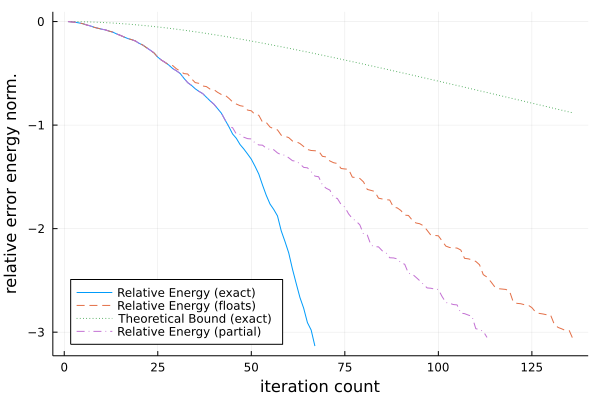
\includegraphics[width=10cm]{fig1.png}
            \caption{
                The relative energy norm error for different methods. Blue solid line: The exact conjugate gradient convergence. Purple dotdashed: The conjugate gradient that is partially orthgonalized with previous 32 residual and conjugate vectors. organed dashed: the Original conjugate gradient. Green dot: The tighter theretical upper bound derived by chebyshev (4.3.20). For this plot: $\rho = 0.9$, the matrix is $256\times 256$. 
            }
        \end{figure}
        The Chebyshev bound is no longer a tight bound because the distribution of the eigenvalues are not perfectly uniform. The partially orthogonalized methods diverges from the exact error after more steps of iterations compare to the relative error without any orthogonalizations. These are seemed in \hyperref[fig:1]{(fig 1)}. 
        \begin{remark}
            The convergence is disappointing under floating point arithematic and the promised efficiency of the algorithm is not there anymore if the matrix is ill-conditioned. If we were to use a fully re-orthogonalized variant of the CG, the memory needed and the totaly complexity for a fixed tolerance is going to be on the same scale of solving it by direct methods. 
        \end{remark}
    \subsection{Greenbaum's Backward Analysis and Paige's Floating Point Analysis}
        In this section we present the backwards analysis of the algorithm in a more thoroughly manner and exam its consequences. When floating point arithematic is used, the eigenvalues of the Tridiagonal matrices might inttroduces ghost eigenvectors for the Lanczos Iterations, and using the equivalence of the Lanczos iterations and CG, we can capture a posteri bound on how much the error is exactly during the iterations of CG. 
        \subsubsection*{The residual}
            Recall from proposition \hyperref[prop:Lanczos_Vectors_and_Residuals]{Propposition 4.6} that the residual of the CG can be expressed interms of the lanczos vector. However, the Lanczos Algorithm under floating doesn't produces perfectly orthogonal Lanczos Vectors, $\tilde{Q}_k$ is not quiet orthogonal, which would also means that $\tilde{Q}_k^HA\tilde{Q}_k\approx T_k$ where $T_k$ is the results from the Lanczos Algorithm, which is only the truncation of the tridiagonal parts of the matrix $\tilde{Q}_k^HA\tilde{Q}_k$. However when we solve for $y_k$ using the expression $y_k = \beta T^{-1}_k\xi_1$, and this is what the CG algorithm does faithflly. The algorithm still thought $T_k$ produced by itself is still perfectly tridiagonal, but it's actually off because $Q_k$ is not quiet orthogonal, hence the algorithm never quiet find the optimal under the conjugate basis. At this point it might seems that tiny errors to the Lanczos vector is very problematic, but in fact
            using the foolishness of CG and assume that the computation of $y_k$ is exact and it's computed as: $y_k = \beta T^{-1}\xi_1$. That only left us with fewer type of floating errors to keep track of. Next, we proceed to look for the residual of the CG algorithm by assuming that the lanczos recurrences has floating point errors: 
            \begin{align}
                AQ_k = Q_{k + 1} \begin{bmatrix}
                    T_k
                    \\
                    \beta_k \xi_k^T
                \end{bmatrix} + F_k
            \end{align}
            Reader please reflect on the fact that, right now the $Q_k$ and is the EXACT and $T_k$ is produced by the Lanczos Algorithm, and we are fixing the recurrences with $F_k$, a matrix full of floating error to correct it so that the equality holds true. 
            \begin{align}
                r_k &= r_0 - AQ_ky_k
                \\
                r_k &= r_0 - 
                    \left(
                        Q_{k + 1} \begin{bmatrix}
                            T_k
                            \\
                            \beta_k \xi_k^T
                        \end{bmatrix}
                        + 
                        F_k
                    \right)
                y_k
                \\
                r_k &= 
                \underbrace{\left(
                    r_0 - Q_{k + 1}\begin{bmatrix}
                        T_k
                        \\
                        \beta_k \xi_k^T
                    \end{bmatrix}y_k
                \right)}_{= -\beta_k\xi_k^Ty_kq_{k + 1}} + F_k \beta T_k^{-1}\xi_1
                \\
                \implies
                \frac{\Vert r_{k + 1}\Vert}
                {
                    \Vert r_0\Vert
                } &\le
                \beta_k \Vert
                    \xi_k^T T_k^{-1}\xi_1 q_{k + 1}
                \Vert + 
                \Vert F_kT_k^{-1}\xi_1 \Vert
                \\
                \frac{\Vert r_{k + 1}\Vert}
                {
                    \Vert r_0\Vert
                } &= 
                \le 
                \beta_k |
                    \xi_k^T T_k^{-1}\xi_1
                | + 
                \Vert F_k\Vert  \Vert T_k^{-1}\xi_1\Vert
            \end{align}
            Here, because of the assumption of exactness for the $Q_k$ matrices we are able to reuse \hyperref[prop:Lanczos_Vectors_and_Residuals]{Propposition 4.6} to regaudge it and obtain a similar expression but this time, taking the floating error into account. 
        
        \subsubsection{Convergence Rate and Paige's Theorem}
            Now, we introduce a new theorem poposed paige. Which gives a bound to the floating point errors for the Lanczos Algorithm. The theorem goes as follow: 
            \begin{theorem}[Paige's Theorem]
                The eigenvalues $\tau_i^{(j)}, i = 1, \cdots, j$ of the tridiagonal matix $T_j$ satisfies: 
                \begin{align}
                    \lambda_1 - j^{5/2}\epsilon_2\Vert A\Vert 
                    \le \theta_i^{(j)}
                    \le 
                    \lambda_n + j^{5/2}\epsilon_2\Vert A\Vert
                \end{align}
            \end{theorem}
            
        
\section{Appendix}
\newpage
\section{Biliography}
            
            

\end{document}
